%DIF 1-12c1-2
%DIF LATEXDIFF DIFFERENCE FILE
%DIF DEL feb_submission/Paper_SPHfP_feb2020_prb.tex   Fri Apr  3 17:45:17 2020
%DIF ADD sp_hafnium.tex                               Mon Apr 20 19:05:16 2020
%DIF < %%   This file is part of the APS files in the REVTeX 4 distribution.
%DIF < %%   Version 4.1r of REVTeX, August 2010
%DIF < %%
%DIF < %%
%DIF < %%   Copyright (c) 2001, 2009, 2010 The American Physical Society.
%DIF < %%
%DIF < %
%DIF < \documentclass[aps,pra,reprint,groupedaddress]{revtex4-1}
%DIF < 
%DIF < %\documentclass[aps,pra,twocolumn,groupedaddress]{revtex4-1}
%DIF < %\documentclass[aps,prb,reprint,superscriptaddress]{revtex4-1}
%DIF < %%%%%%%%%%%%%%%%%%%%%%%%%%%%%%%%%%%%%%%%%%%%%%%%%%%%%%%%%%%%%%%%%%%%%%%%%%%%%%%%%%%%%%%%%%%%%%%%%%%%%%%%%%%%%%%%%%%%%%%%%%%%
%DIF -------
\documentclass[aps,pra,reprint,superscriptaddress]{revtex4-1} %DIF > 
%\documentclass[aps,pra,reprint,groupedaddress,showpacs,showkeys]{revtex4-1} %DIF > 
%DIF -------
\usepackage{amssymb}
\usepackage{amsthm}
\usepackage{amsmath} 
\usepackage{graphicx}
%DIF 17a7-9
\usepackage{soul} %DIF > 
\usepackage{xcolor} %DIF > 
\setstcolor{red} %DIF > 
%DIF -------
\usepackage[mathlines]{lineno}% Enable numbering of text and display math
%\linenumbers\relax % Commence numbering lines


%DIF < %\def\clau#1{\textcolor{ForestGreen}{#1}}
%DIF -------
\def\clau#1{\textcolor{red}{#1}} %DIF > 
%DIF < %\def\minor#1{\textcolor{green}{#1}}
\def\duda#1{\textcolor{green}{#1}} %DIF > 
\def\ale#1{\textcolor{blue}{#1}} %DIF > 
%DIF PREAMBLE EXTENSION ADDED BY LATEXDIFF
%DIF UNDERLINE PREAMBLE %DIF PREAMBLE
\RequirePackage[normalem]{ulem} %DIF PREAMBLE
\RequirePackage{color}\definecolor{RED}{rgb}{1,0,0}\definecolor{BLUE}{rgb}{0,0,1} %DIF PREAMBLE
\providecommand{\DIFadd}[1]{{\protect\color{blue}\uwave{#1}}} %DIF PREAMBLE
\providecommand{\DIFdel}[1]{{\protect\color{red}\sout{#1}}}                      %DIF PREAMBLE
%DIF SAFE PREAMBLE %DIF PREAMBLE
\providecommand{\DIFaddbegin}{} %DIF PREAMBLE
\providecommand{\DIFaddend}{} %DIF PREAMBLE
\providecommand{\DIFdelbegin}{} %DIF PREAMBLE
\providecommand{\DIFdelend}{} %DIF PREAMBLE
%DIF FLOATSAFE PREAMBLE %DIF PREAMBLE
\providecommand{\DIFaddFL}[1]{\DIFadd{#1}} %DIF PREAMBLE
\providecommand{\DIFdelFL}[1]{\DIFdel{#1}} %DIF PREAMBLE
\providecommand{\DIFaddbeginFL}{} %DIF PREAMBLE
\providecommand{\DIFaddendFL}{} %DIF PREAMBLE
\providecommand{\DIFdelbeginFL}{} %DIF PREAMBLE
\providecommand{\DIFdelendFL}{} %DIF PREAMBLE
\newcommand{\DIFscaledelfig}{0.5}
%DIF HIGHLIGHTGRAPHICS PREAMBLE %DIF PREAMBLE
\RequirePackage{settobox} %DIF PREAMBLE
\RequirePackage{letltxmacro} %DIF PREAMBLE
\newsavebox{\DIFdelgraphicsbox} %DIF PREAMBLE
\newlength{\DIFdelgraphicswidth} %DIF PREAMBLE
\newlength{\DIFdelgraphicsheight} %DIF PREAMBLE
% store original definition of \includegraphics %DIF PREAMBLE
\LetLtxMacro{\DIFOincludegraphics}{\includegraphics} %DIF PREAMBLE
\newcommand{\DIFaddincludegraphics}[2][]{{\color{blue}\fbox{\DIFOincludegraphics[#1]{#2}}}} %DIF PREAMBLE
\newcommand{\DIFdelincludegraphics}[2][]{% %DIF PREAMBLE
\sbox{\DIFdelgraphicsbox}{\DIFOincludegraphics[#1]{#2}}% %DIF PREAMBLE
\settoboxwidth{\DIFdelgraphicswidth}{\DIFdelgraphicsbox} %DIF PREAMBLE
\settoboxtotalheight{\DIFdelgraphicsheight}{\DIFdelgraphicsbox} %DIF PREAMBLE
\scalebox{\DIFscaledelfig}{% %DIF PREAMBLE
\parbox[b]{\DIFdelgraphicswidth}{\usebox{\DIFdelgraphicsbox}\\[-\baselineskip] \rule{\DIFdelgraphicswidth}{0em}}\llap{\resizebox{\DIFdelgraphicswidth}{\DIFdelgraphicsheight}{% %DIF PREAMBLE
\setlength{\unitlength}{\DIFdelgraphicswidth}% %DIF PREAMBLE
\begin{picture}(1,1)% %DIF PREAMBLE
\thicklines\linethickness{2pt} %DIF PREAMBLE
{\color[rgb]{1,0,0}\put(0,0){\framebox(1,1){}}}% %DIF PREAMBLE
{\color[rgb]{1,0,0}\put(0,0){\line( 1,1){1}}}% %DIF PREAMBLE
{\color[rgb]{1,0,0}\put(0,1){\line(1,-1){1}}}% %DIF PREAMBLE
\end{picture}% %DIF PREAMBLE
}\hspace*{3pt}}} %DIF PREAMBLE
} %DIF PREAMBLE
\LetLtxMacro{\DIFOaddbegin}{\DIFaddbegin} %DIF PREAMBLE
\LetLtxMacro{\DIFOaddend}{\DIFaddend} %DIF PREAMBLE
\LetLtxMacro{\DIFOdelbegin}{\DIFdelbegin} %DIF PREAMBLE
\LetLtxMacro{\DIFOdelend}{\DIFdelend} %DIF PREAMBLE
\DeclareRobustCommand{\DIFaddbegin}{\DIFOaddbegin \let\includegraphics\DIFaddincludegraphics} %DIF PREAMBLE
\DeclareRobustCommand{\DIFaddend}{\DIFOaddend \let\includegraphics\DIFOincludegraphics} %DIF PREAMBLE
\DeclareRobustCommand{\DIFdelbegin}{\DIFOdelbegin \let\includegraphics\DIFdelincludegraphics} %DIF PREAMBLE
\DeclareRobustCommand{\DIFdelend}{\DIFOaddend \let\includegraphics\DIFOincludegraphics} %DIF PREAMBLE
\LetLtxMacro{\DIFOaddbeginFL}{\DIFaddbeginFL} %DIF PREAMBLE
\LetLtxMacro{\DIFOaddendFL}{\DIFaddendFL} %DIF PREAMBLE
\LetLtxMacro{\DIFOdelbeginFL}{\DIFdelbeginFL} %DIF PREAMBLE
\LetLtxMacro{\DIFOdelendFL}{\DIFdelendFL} %DIF PREAMBLE
\DeclareRobustCommand{\DIFaddbeginFL}{\DIFOaddbeginFL \let\includegraphics\DIFaddincludegraphics} %DIF PREAMBLE
\DeclareRobustCommand{\DIFaddendFL}{\DIFOaddendFL \let\includegraphics\DIFOincludegraphics} %DIF PREAMBLE
\DeclareRobustCommand{\DIFdelbeginFL}{\DIFOdelbeginFL \let\includegraphics\DIFdelincludegraphics} %DIF PREAMBLE
\DeclareRobustCommand{\DIFdelendFL}{\DIFOaddendFL \let\includegraphics\DIFOincludegraphics} %DIF PREAMBLE
%DIF END PREAMBLE EXTENSION ADDED BY LATEXDIFF

\begin{document}

%Title of paper
\title{The stopping power of \DIFaddbegin \DIFadd{hydrogen in }\DIFaddend hafnium and \DIFaddbegin \\
\DIFaddend the importance of relativistic $4f$ electrons}
%Authors and affiliations

%---------------------------Argentina
\author{C. C. Montanari}
\email{mclaudia@iafe.uba.ar}
\affiliation{Instituto de Astronom\'{\i}a y F\'{\i}sica del Espacio, 
Consejo Nacional de Investigaciones Cient\'{\i}ficas y T\'{e}cnicas - 
Universidad de Buenos Aires, Pabell\'on IAFE, 1428 Buenos Aires, 
Argentina}
%DIF < 
%DIF < \affiliation{Universidad de Tres de Febrero, Sáenz Peña, Buenos Aires, Argentina.}
%DIF < ------------------------------
\DIFaddbegin 

%DIF > ---------------------------Chile
\author{\DIFadd{P. A. Miranda}}
\affiliation{Departamento de F\'isica, Facultad de Ciencias Naturales, 
Matem\'atica y del Medio Ambiente. Universidad Tecnol\'ogica Metropolitana. 
7800002, Chile}
%DIF > -------------------------Lisboa
\author{\DIFadd{E. Alves}}
\affiliation{Centro de Ci\^{e}ncias e Tecnologias Nucleares, Instituto 
Superior T\'ecnico, Universidade de Lisboa, 2696-953 Sacav\'{e}m, 
Portugal}
\affiliation{Instituto de Plasma e Fus\~{a}o Nuclear, Instituto Superior 
T\'ecnico, Universidade de Lisboa, 2696-953 Sacav\'{e}m, Portugal}

%DIF > ------------------------------Argentina
\DIFaddend \author{A. M. P. Mendez}
\affiliation{Instituto de Astronom\'{\i}a y F\'{\i}sica del Espacio, 
Consejo Nacional de Investigaciones Cient\'{\i}ficas y T\'{e}cnicas - 
Universidad de Buenos Aires, Pabell\'on IAFE, 1428 Buenos Aires, 
Argentina}
%DIF < 
%-------------------------------
\author{D. M. Mitnik}
\affiliation{Instituto de Astronom\'{\i}a y F\'{\i}sica del Espacio, 
Consejo Nacional de Investigaciones Cient\'{\i}ficas y T\'{e}cnicas - 
Universidad de Buenos Aires, Pabell\'on IAFE, 1428 Buenos Aires, 
Argentina}
%DIF < 
%DIF < \affiliation{Universidad de Buenos Aires, Facultad de Ciencias Exactas y Naturales, Departamento de F\'{\i}sica, Ciudad Universitaria, 1428 Buenos Aires, Argentina.}
%----------------------------------------------
\author{J. E. Miraglia}
\affiliation{Instituto de Astronom\'{\i}a y F\'{\i}sica del Espacio, 
Consejo Nacional de Investigaciones Cient\'{\i}ficas y T\'{e}cnicas - 
Universidad de Buenos Aires, Pabell\'on IAFE, 1428 Buenos Aires, 
Argentina}
%DIF < 
%DIF < ---------------------------Chile

\DIFdelbegin %DIFDELCMD < \author{P.A. Miranda}
%DIFDELCMD < \affiliation{Departmento de F\'isica, Facultad de Ciencias Naturales, Matem\'atica y del Medio Ambiente. Universidad Tecnol\'ogica Metropolitana. 7800002, Chile}
%DIFDELCMD < %%%
%DIF < ----------------------------
\DIFdelend %DIF > ---------------------------- Chile
\author{R. Correa}
\DIFdelbegin %DIFDELCMD < \affiliation{Departmento de F\'isica, Facultad de Ciencias Naturales, Matem\'atica y del Medio Ambiente. Universidad Tecnol\'ogica Metropolitana. 7800002, Chile}
%DIFDELCMD < %%%
\DIFdelend \DIFaddbegin \affiliation{Departamento de F\'isica, Facultad de Ciencias Naturales, 
Matem\'atica y del Medio Ambiente. Universidad Tecnol\'ogica Metropolitana. 
7800002, Chile}
%DIF > ----------------------------
\DIFaddend \author{J. Wachter}
\DIFdelbegin %DIFDELCMD < \affiliation{Departmento de F\'isica, Facultad de Ciencias Naturales, Matem\'atica y del Medio Ambiente. Universidad Tecnol\'ogica Metropolitana. 7800002, Chile}
%DIFDELCMD < %%%
\DIFdelend \DIFaddbegin \affiliation{Departamento de F\'isica, Facultad de Ciencias Naturales, 
Matem\'atica y del Medio Ambiente. Universidad Tecnol\'ogica Metropolitana. 
7800002, Chile}
%DIF > ----------------------------
\DIFaddend \author{M. Aguilera}
\DIFdelbegin %DIFDELCMD < \affiliation{Departmento de F\'isica, Facultad de Ciencias Naturales, Matem\'atica y del Medio Ambiente. Universidad Tecnol\'ogica Metropolitana. 7800002, Chile}
%DIFDELCMD < %%%
\DIFdelend \DIFaddbegin \affiliation{Departamento de F\'isica, Facultad de Ciencias Naturales, 
Matem\'atica y del Medio Ambiente. Universidad Tecnol\'ogica Metropolitana. 
7800002, Chile}

\DIFaddend %-------------------------Lisboa
\DIFdelbegin %DIFDELCMD < \author{E. Alves}
%DIFDELCMD < \affiliation{Centro de Ci\^{e}ncias e Tecnologias Nucleares, Instituto Superior T\'ecnico, Universidade de Lisboa,
%DIFDELCMD < 2696-953 Sacav\'{e}m, Portugal}
%DIFDELCMD < \affiliation{Instituto de Plasma e Fus\~{a}o Nuclear, Instituto Superior T\'ecnico, Universidade de Lisboa, 2696-953 Sacav\'{e}m, Portugal}
%DIFDELCMD < %%%
%DIF < ---------------------------
\DIFdelend \author{N. Catarino}
\affiliation{Centro de Ci\^{e}ncias e Tecnologias Nucleares, Instituto 
Superior T\'ecnico, Universidade de Lisboa, 2696-953 Sacav\'{e}m, 
Portugal}
%---------------------------
\author{R. C. da Silva}
\affiliation{Centro de Ci\^{e}ncias e Tecnologias Nucleares, Instituto 
Superior T\'ecnico, Universidade de Lisboa, 2696-953 Sacav\'{e}m, 
Portugal}

\date{\today}

%DIF < =============================================================================================================================================================================================
%DIF < =============================================================================================================================================================================================
%DIF > =======================================================================
%DIF > =======================================================================
\begin{abstract}
 The stopping power of protons through Hf foil has been studied both 
experimentally and theoretically. The measurements were performed at 
the Laboratory of Accelerators and X-Ray Diffraction in Lisbon \DIFdelbegin \DIFdel{, }\DIFdelend by 
using the transmission method on self-supporting stopping material. 
 The overall uncertainty of around $5\%$ was established over the 
protons energy range  (0.6-2.5) MeV. The theoretical developments 
involved fully relativistic atomic structure calculations for Hf, which 
required the solution of the Dirac equation. The shell-wise local plasma 
approximation (SLPA) was used to describe the energy transferred to the 
bound $1s$-$4f$ electrons, and the outer four electrons were considered 
as a free electron gas (FEG). We found the relativistic description of 
the $4f$-shell and the screening between $4f$ and $5p$ electrons \DIFdelbegin \DIFdel{are }\DIFdelend \DIFaddbegin \DIFadd{to be 
}\DIFaddend decisive around the stopping maximum. Present theoretical and 
experimental results are in \DIFdelbegin \DIFdel{very good }\DIFdelend \DIFaddbegin \DIFadd{excellent }\DIFaddend agreement in the energy region 
of the new measurements. However, \DIFdelbegin \DIFdel{the present }\DIFdelend \DIFaddbegin \DIFadd{our }\DIFaddend theoretical stopping 
cross sections show substantial differences with the most used 
semi-empirical models (SRIM2013 and ICRU-49) at intermediate to low 
energies. Our calculations suggest the stopping maximum \DIFaddbegin \DIFadd{to be }\DIFaddend higher and 
shifted to lower energies than these previous predictions. Future 
measurements below 100 keV would be \DIFdelbegin \DIFdel{decisive }\DIFdelend \DIFaddbegin \DIFadd{necessary }\DIFaddend for a better \DIFdelbegin \DIFdel{knowledge  }\DIFdelend \DIFaddbegin \DIFadd{understanding 
of the stopping power }\DIFaddend around the maximum and below.
\end{abstract}

% insert suggested PACS numbers in braces on next line
\pacs{34.50.Bw} \keywords{Stopping power, hafnium, Relativistic atomic 
structure, Transmission method}

\maketitle

%DIF < \linenumbers
%DIF < =============================================================================================================================================================================================
%DIF < =============================================================================================================================================================================================
\DIFaddbegin \linenumbers
%DIF > =======================================================================
%DIF > =======================================================================
\DIFaddend \section{Introduction}
\label{intro}

For impact energies above a few keV/amu, mono-energetic charged 
particles penetrating a foil of any material lose their energy through 
a series of consecutive inelastic collisions, mainly with target 
electrons~\cite{Chu01,Sigmund}. The information given by the energy 
loss process is essential not only to have a better \DIFdelbegin \DIFdel{knowledge }\DIFdelend \DIFaddbegin \DIFadd{comprehension }\DIFaddend of the 
physics behind the fundamental interactions \DIFdelbegin \DIFdel{, }\DIFdelend but also because it plays 
\DIFdelbegin \DIFdel{an important }\DIFdelend \DIFaddbegin \DIFadd{a vital }\DIFaddend role in many applied fields such as materials science, 
nuclear physics, ionic implantation\DIFaddbegin \DIFadd{, }\DIFaddend and radiotherapy~\cite{Sigmund,Schardt}. 
Experimental data on ion mean energy loss per unit path $S(E)$ is of 
crucial relevance to check the reliability of semi-empirical models and 
to determine some key parameters~\cite{Diwan,Damache04,Damache02}. The 
experimental data available is often rather scarce, which is troublesome 
when the material under study corresponds to an element of low 
occurrence on the Earth's upper crust, such as hafnium.

So far, only one experimental work has been published regarding the 
stopping power cross section of pure hafnium for protons~\cite{Sirotinin}, 
while more attention has been recently given to studies involving 
hafnium oxide due to its practical use~\DIFdelbegin \DIFdel{\mbox{%DIFAUXCMD
\cite{Abril,Behar,Primetzhofer}}\hspace{0pt}%DIFAUXCMD
}\DIFdelend \DIFaddbegin \DIFadd{\mbox{%DIFAUXCMD
\cite{Abril,Behar,Primetzhofer,Roth}}\hspace{0pt}%DIFAUXCMD
}\DIFaddend . 
It is well known that significant attention has been paid in recent 
years to transition metal-oxides such as HfO$_2$ because of their 
potential as alternative gate dielectrics to replace SiO$_2$ for the 
future generation of nano-electronics with less than 45 nm gate 
length~\cite{Choi,Robertson}. Some important physical properties of the 
above mentioned metal-oxide films depend on \DIFdelbegin \DIFdel{its }\DIFdelend \DIFaddbegin \DIFadd{their }\DIFaddend thickness, which is 
often measured by using Rutherford Backscattering 
Spectrometry~\cite{Alfassi01,Tesmer01}\DIFdelbegin \DIFdel{, a method that }\DIFdelend \DIFaddbegin \DIFadd{. This method }\DIFaddend relies heavily on 
the determination of the stopping power of ion beams in the material of 
interest.

In this study, we report experimental stopping power cross sections over 
the incident energy range (0.6-2.5) MeV for protons crossing 
self-supported Hf thin-film by using the transmission method. We aim not 
only to upgrade stopping power data compilations~\cite{HPaul03,mondim17} 
but also to provide useful information about the processes governing the 
slowing down of protons in multi-electronic targets. In the rare earth 
metals, the $4f$ electrons play \DIFdelbegin \DIFdel{a relevant }\DIFdelend \DIFaddbegin \DIFadd{an essential }\DIFaddend role in the stopping power 
\DIFdelbegin \DIFdel{, being }\DIFdelend \DIFaddbegin \DIFadd{since they belong to }\DIFaddend the first shell of bound electrons below the 
conduction band. As already noted \DIFdelbegin \DIFdel{~}\DIFdelend \cite{Roth17}, the free electron gas 
(FEG) shows unexpected %DIF < a peculiar
behavior in these elements, which casts %DIF < that states 
doubts 
on its proper description. In the case of Hf, we found the contribution 
of the $4f$-shell \DIFaddbegin \DIFadd{to be }\DIFaddend decisive even at impact energies around the 
stopping maximum, as \DIFaddbegin \DIFadd{will be }\DIFaddend shown later.

The theoretical approach implemented in this work uses the shell-wise 
local plasma approximation (SLPA)~\cite{mon13} to describe the energy 
transferred to the bound $1s$-$4f$ electrons \DIFdelbegin \DIFdel{, }\DIFdelend and two different models 
for the FEG\DIFdelbegin \DIFdel{: }\DIFdelend \DIFaddbegin \DIFadd{; in low energy region, }\DIFaddend the screened potential with cusp 
condition model (SPCC)~\cite{mon17}, which is non-linear binary 
formalism%DIF < ,  for energies below that of the plasmon excitation
\DIFdelbegin \DIFdel{; }\DIFdelend \DIFaddbegin \DIFadd{, }\DIFaddend and the Mermin-Lindhard dielectric formalism 
(ML)~\cite{Mermin} \DIFdelbegin \DIFdel{, }\DIFdelend for energies around the stopping maximum and above. 
Our model requires the relativistic wave functions and binding energies 
of Hf \DIFdelbegin \DIFdel{, and considers 4 }\DIFdelend \DIFaddbegin \DIFadd{and considers four }\DIFaddend electrons per atom in the FEG~\cite{mendez2019}. 
%DIF < On the other hand,
\DIFdelbegin \DIFdel{Hf has the extra interest of }\DIFdelend \DIFaddbegin \DIFadd{Hafnium is particularly interesting since }\DIFaddend the filled $4f$-subshell (with 
14 electrons) \DIFdelbegin \DIFdel{as the main contribution }\DIFdelend \DIFaddbegin \DIFadd{is the main contributor }\DIFaddend below the FEG, causing the 
stopping cross sections to be very sensitive to a good description of 
this shell. The screening among the $4f$ and $5p$ electrons has been 
considered and found to play a \DIFdelbegin \DIFdel{major }\DIFdelend \DIFaddbegin \DIFadd{significant }\DIFaddend role within the SLPA 
calculations.

The experimental details and data are given in Section~\ref{experiment}, 
while the theoretical method is explained in Section~\ref{theory}. 
Present theoretical and experimental values are finally compared to the 
\DIFdelbegin \DIFdel{available experimental values ~\mbox{%DIFAUXCMD
\cite{Sirotinin}}\hspace{0pt}%DIFAUXCMD
, the ICRU-49 calculations~\mbox{%DIFAUXCMD
\cite{ICRU49} }\hspace{0pt}%DIFAUXCMD
and }\DIFdelend \DIFaddbegin \DIFadd{only experimental values measured by Sirotinin }{\it \DIFadd{et al.}}\DIFadd{~\mbox{%DIFAUXCMD
\cite{Sirotinin}  
}\hspace{0pt}%DIFAUXCMD
with the backscattering method, the theoretical results by Grande and 
Schiwietz~\mbox{%DIFAUXCMD
\cite{Grande,casp52}}\hspace{0pt}%DIFAUXCMD
, and by Sigmund and Schinner~\mbox{%DIFAUXCMD
\cite{DPASS20}}\hspace{0pt}%DIFAUXCMD
, 
and also with the semi-empirical values from }\DIFaddend the SRIM-2013 
package~\cite{Ziegler01} \DIFaddbegin \DIFadd{and the ICRU-49 tabulation~\mbox{%DIFAUXCMD
\cite{ICRU49}}\hspace{0pt}%DIFAUXCMD
}\DIFaddend . 
Conclusions and discussions are given in Section~\ref{conclusion}. All 
the present data can be found at the Zenodo platform \DIFdelbegin \DIFdel{~}\DIFdelend \cite{zenodo}.

%DIF < =============================================================================================================================================================================================
\DIFdelbegin %DIFDELCMD < 

%DIFDELCMD < %%%
\DIFdelend %DIF > -----------------------------------------------------------------------
\begin{figure}[!t]
\centering
\includegraphics[width=9cm]{Fig01.eps}
\caption{RBS spectrum for $E_{\mathrm{avg}}=921.1$ keV protons on 
\DIFaddbeginFL \DIFaddFL{the }\DIFaddendFL hafnium sample\DIFaddbeginFL \DIFaddFL{, }\DIFaddendFL which is subsequently used to determine the energy 
loss in the foil.}
\label{F01}
\end{figure}


%DIF < =============================================================================================================================================================================================
\DIFdelbegin %DIFDELCMD < 

%DIFDELCMD < %%%
\DIFdelend %DIF > =======================================================================
\section{EXPERIMENTAL ARRANGEMENTS}
\label{experiment}
\DIFaddbegin 

%DIF > -----------------------------------------------------------------------
\DIFaddend \subsection{Accelerator and scattering Chamber}
The procedure used in this work to obtain stopping power data is 
essentially the same as described in Ref.~\cite{Miranda01}. The present 
measurements were made at the IST/LATR (Laboratory of Accelerators and 
X-Ray Diffraction) in Lisbon. This facility uses a 2.5 MV Van de Graaff 
accelerator to deliver $^1$H$^+$ primary ion beams through a series of 
electrostatic lenses and collimators onto a thin Au/SiO$_2$ sample\DIFaddbegin \DIFadd{, 
}\DIFaddend which is used as a scattering center. This sample was placed in the 
center of \DIFdelbegin \DIFdel{a }\DIFdelend \DIFaddbegin \DIFadd{an }\DIFaddend RBS/C scattering chamber, where a high vacuum (pressure of 
$\sim$10$^{-6}$ Torr) was maintained during the measurements. The beam 
current on the sample was kept at around 5.0 nA to attain sufficient 
statistics in each particle spectrum. By using a beam spot of about 
1.0 mm in diameter, a solid angle of 11.4 msr was attained. The overall 
energy resolution (FWHM) of the detection system was about 15 keV 
relative to 5.486 MeV alpha particles from a $^{241}$Am source.

%DIF < ---------------------------------------------------------------------------------------------------------------------------------------------------------------------------------------------
%DIF > -----------------------------------------------------------------------
\subsection{Target}
The stopping material under analysis was a hafnium foil with \DIFaddbegin \DIFadd{a }\DIFaddend nominal 
thickness of 1.0 $\mu$m and 99.95\% purity\DIFaddbegin \DIFadd{, }\DIFaddend which was supplied by Lebow 
Company~\cite{Lebow}. However, a more precise thickness value was 
achieved by measuring the energy loss of alpha particles coming from a 
calibrated ($^{239}$Pu, $^{241}$Am, $^{244}$Cm) source. From the alpha 
spectra with and without the Hf foil interposed, the characteristic 
energy shift $\delta$E was measured and then combined with the stopping 
power for 5.486 MeV alphas on hafnium (55.69 eV/$10^{15}$ at/cm$^2$) 
found in Ref.~\cite{Ziegler01} to obtain an areal density of 
($4.13 \pm 0.21$)$\times 10^{19}$ at/cm$^2$\DIFaddbegin \DIFadd{, }\DIFaddend which corresponds to a 
thickness of $0.920\pm0.046 \mu$m.
%DIF < ---------------------------------------------------------------------------------------------------------------------------------------------------------------------------------------------
\DIFaddbegin 

%DIF > -----------------------------------------------------------------------
\DIFaddend \subsection{Energy loss measurement}
Once the beam impinges on the Au/SiO$_2$ sample, protons are 
\DIFdelbegin \DIFdel{back-scattered }\DIFdelend \DIFaddbegin \DIFadd{backscattered }\DIFaddend towards a Si surface barrier detector located at 
140$^{\circ}$ relative to the initial beam direction. Fig.~\ref{F01} 
shows two particle spectra\DIFdelbegin \DIFdel{where }\DIFdelend \DIFaddbegin \DIFadd{, where the }\DIFaddend ion energies $E_2$ and $E_1$ are 
associated \DIFdelbegin \DIFdel{to }\DIFdelend \DIFaddbegin \DIFadd{with }\DIFaddend a placed and removed hafnium sample, respectively. Both 
energy distributions were fitted by Gaussian functions to obtain the 
mean energy and width (FWHM) of the peaks \DIFdelbegin \DIFdel{~}\DIFdelend \cite{Sun01}, and from the 
difference between these two peak positions in the spectrum, the total 
energy loss $\Delta E = (E_1 - E_2)$ in the foil was calculated. As 
established in previous studies \DIFdelbegin \DIFdel{~}\DIFdelend \cite{Miranda01,Damache02}, the 
experimental stopping power cross sections $\varepsilon (E) $ are 
determined at some mean energy $E_{\mathrm{avg}}$ by measuring the ion 
energy losses $\Delta E$ within the investigated Hf foil, which has a 
mean thickness denoted by $\Delta x$. In this way, only when the energy 
loss fraction $\Delta E/E_{\mathrm{avg}}$ across the Hf foil is not 
exceeding 20\%\DIFaddbegin \DIFadd{, }\DIFaddend it is possible to define the stopping cross section by 
\DIFdelbegin \DIFdel{~}\DIFdelend \cite{Raisanen01,Schulz01}:
\begin{equation}\label{eq:stcross}
 \varepsilon(E)=\frac{S(E)}{N}=-\frac{dE}{N\,dx}\approx-\frac{\Delta E}{N\Delta x},
\end{equation}
where $N$ denotes the atomic number density (atoms cm$^{-3}$) of the 
material under study. When this condition was not fulfilled, a small 
correction to the mean energies $E_{\mathrm{avg}}$ was applied in order 
to account for the \DIFdelbegin \DIFdel{nonlinear }\DIFdelend \DIFaddbegin \DIFadd{non-linear }\DIFaddend dependence on ion energy of stopping 
powers \DIFdelbegin \DIFdel{~}\DIFdelend \cite{Chilton,Rajatora}.


%DIF > =======================================================================
\section{Theoretical Method} 
\label{theory}
The energy loss of ions in metal targets responds to different physical 
mechanisms, depending on the impact ion velocity. At low velocities, the 
binary collisions are responsible for the loss of energy by the ion. 
The main contribution is the ionization of electrons of the metal 
conduction band, which is well approximated by a free electron gas (FEG) 
of Fermi velocity $v_F$. Above \DIFdelbegin \DIFdel{certain velocity }\DIFdelend \DIFaddbegin \DIFadd{a particular velocity value }\DIFaddend (i.e.\DIFaddbegin \DIFadd{, 
}\DIFaddend $v\geq 1.5\,v_F$), not only binary but also collective excitations 
(plasmons) \DIFdelbegin \DIFdel{are possible}\DIFdelend \DIFaddbegin \DIFadd{occur}\DIFaddend ~\cite{mon17}. Moreover, at high energies, also the 
bound electrons contribute to the stopping power. The method used in 
this work combines a \DIFaddbegin \DIFadd{FEG }\DIFaddend description for the interaction with the 
valence (or conduction) electrons \DIFdelbegin \DIFdel{as a FEG, }\DIFdelend and a different one for the 
interaction with the bound electrons.

We used the SPCC model~\cite{mon17} to describe the stopping power of 
low velocity charged particles in the FEG. It is a non-perturbative 
binary collisional approximation, thus valid at energies below that of 
plasmon excitations.  The SPCC~\cite{mon17} is based on a screened 
central potential with cusp condition of the electronic density close 
to the projectile. This model proved to give a good description of the 
induced electron density even for negative projectiles~\cite{mon17} 
\DIFdelbegin \DIFdel{, }\DIFdelend and reproduces the low velocity proton-antiproton differences in the 
stopping power (Barkas effect). The SPCC formalism only depends on the 
Wigner-Seitz radio, $r_S$, which is a measure of the electronic density 
of the FEG. For metals of well-known $r_S$, the SPCC describes \DIFdelbegin \DIFdel{correctly }\DIFdelend the low 
energy experimental stopping data \DIFaddbegin \DIFadd{correctly}\DIFaddend ~\cite{mon17}, agreeing with 
the DFT results by Echenique and coworkers~\cite{eche81,nagy89} at $v=0$. 

%DIF < In the case of 
Hafnium ($Z=72$, [Xe] $4f^{14}\,6s^2\,5d_{3/2}^1\,5d_{5/2}^1$) \DIFdelbegin \DIFdel{, }\DIFdelend belongs 
to the first groups of transition metals, with \DIFdelbegin \DIFdel{4 }\DIFdelend \DIFaddbegin \DIFadd{four }\DIFaddend electrons as FEG 
(\DIFdelbegin \DIFdel{theoretical }\DIFdelend $r_S=2.14$ a.u.) and $1s$-$4f$ electrons bound. We compared the 
computed $r_S$ with the experimental value obtained from \DIFaddbegin \DIFadd{the }\DIFaddend measured 
energy loss function by Lynch \textit{et al\DIFaddbegin \DIFadd{.}\DIFaddend }~\cite{lynch75}. The 
experimental plasmon energy of Hf is $\hbar\omega_P \approx 15.8$ eV, 
with a width at half maximum \DIFdelbegin \DIFdel{$\delta \approx 4.4$ }\DIFdelend \DIFaddbegin \DIFadd{$\delta\approx 4.4$ }\DIFaddend eV, and 
\DIFdelbegin \DIFdel{$r_S \approx 2.07$ }\DIFdelend \DIFaddbegin \DIFadd{$r_S\approx 2.07$ }\DIFaddend a.u.~\cite{lynch75}. The difference of less than 
$5\%$ between theoretical and experimental $r_S$ assess Hf as a 
canonical target~\cite{mon17}.

Above certain impact velocity, the plasmon contribution is \DIFdelbegin \DIFdel{important }\DIFdelend \DIFaddbegin \DIFadd{essential
}\DIFaddend (i.e.\DIFaddbegin \DIFadd{, }\DIFaddend around and above the stopping maximum). \DIFdelbegin \DIFdel{An interesting value }\DIFdelend \DIFaddbegin \DIFadd{A value of interest }\DIFaddend for 
our analysis is the minimum impact velocity to excite plasmons, $v_P$. 
In the dielectric formalism, this value can be obtained as 
$v_P\,\approx\,v_F[1+(3\pi\,v_F)^{-1/2}]$~\cite{suppression}. To 
describe the energy loss considering collective and binary excitation, 
we resort to the ML dielectric formalism \DIFdelbegin \DIFdel{~}\DIFdelend \cite{Mermin}, which is a 
linear response, perturbative approximation, so it depends on the 
square of the ion charge. In this formalism, the response of target 
electrons to the ion passage is described through the quantum dielectric 
function, \DIFdelbegin \DIFdel{depending }\DIFdelend \DIFaddbegin \DIFadd{which depends }\DIFaddend on the characteristic $r_S$ and $\delta$ parameters 
of the FEG. 

%----------------------------------------------------------------------
\begin{figure*}[!t]
\centering
\includegraphics[width=11.cm]{bindener.eps}
%DIF <  \includegraphics[width=13.cm]{Hf_bindener_ratio.eps}
\caption{(a) Binding energies of Hf. \DIFdelbeginFL \DIFdelFL{Non-relativistic and }\DIFdelendFL \DIFaddbeginFL \DIFaddFL{Present }\DIFaddendFL relativistic \DIFdelbeginFL \DIFdelFL{calculations }\DIFdelendFL \DIFaddbeginFL \DIFaddFL{and available 
non-relativistic~\mbox{%DIFAUXCMD
\cite{badnell97} }\hspace{0pt}%DIFAUXCMD
values }\DIFaddendFL are given with filled symbols. 
Experimental measurements for solids\DIFaddbeginFL \DIFaddFL{~}\DIFaddendFL \cite{williams1995} are depicted 
with \DIFdelbeginFL \DIFdelFL{hollow }\DIFdelendFL \DIFaddbeginFL \DIFaddFL{open }\DIFaddendFL circles. (b) Corresponding relative errors \DIFaddbeginFL \DIFaddFL{with }\DIFaddendFL respect to 
experimental data.}
\label{Binding_E}
\end{figure*}
%------------------------------------------------------------------------

For the stopping power due to bound electrons, the SLPA~\cite{mon17,mon13} 
is employed. It is worth \DIFdelbegin \DIFdel{to mention }\DIFdelend \DIFaddbegin \DIFadd{mentioning }\DIFaddend that the only inputs for the SLPA 
are the space-dependent densities of each shell in the ground state, 
and their binding energies. Collective processes and screening among 
electrons are included. \DIFdelbegin \DIFdel{Hafnium }\DIFdelend \DIFaddbegin \DIFadd{Since hafnium }\DIFaddend is a relativistic target, \DIFdelbegin \DIFdel{therefore }\DIFdelend the wave 
functions and binding energies must be obtained by solving the \DIFdelbegin \DIFdel{many–electron }\DIFdelend \DIFaddbegin \DIFadd{many-electron 
}\DIFaddend Dirac Hamiltonian. Details of these calculations \DIFaddbegin \DIFadd{and a table of binding 
energies }\DIFaddend have been published in \DIFaddbegin \DIFadd{Ref.}\DIFaddend ~\cite{mendez2019}, \DIFdelbegin \DIFdel{and the }\DIFdelend \DIFaddbegin \DIFadd{while }\DIFaddend Slater-type 
orbital expansions \DIFdelbegin \DIFdel{in}\DIFdelend \DIFaddbegin \DIFadd{are given in Ref.}\DIFaddend ~\cite{Hf_arxiv}.

\DIFdelbegin \DIFdel{Too }\DIFdelend \DIFaddbegin \DIFadd{To }\DIFaddend assess the importance of \DIFdelbegin \DIFdel{the }\DIFdelend \DIFaddbegin \DIFadd{a fully relativistic }\DIFaddend description of bound 
electrons, Fig.~\ref{Binding_E}\DIFdelbegin \DIFdel{shows }\DIFdelend \DIFaddbegin \DIFadd{~}\DIFaddend (a) \DIFdelbegin \DIFdel{non-relativistic~\mbox{%DIFAUXCMD
\cite{badnell97} }\hspace{0pt}%DIFAUXCMD
and our relativistic }\DIFdelend \DIFaddbegin \DIFadd{shows our }\DIFaddend binding energies, 
$E_{nl\pm}$, with $\pm=j\pm1/2$; \DIFdelbegin \DIFdel{and (b) the relative errors with respect to the }\DIFdelend \DIFaddbegin \DIFadd{non-relativistic values~\mbox{%DIFAUXCMD
\cite{badnell97}}\hspace{0pt}%DIFAUXCMD
; 
and }\DIFaddend experimental data on \DIFdelbegin \DIFdel{solid }\DIFdelend \DIFaddbegin \DIFadd{solid-state }\DIFaddend Hf~\cite{williams1995}\DIFdelbegin \DIFdel{from }\DIFdelend \DIFaddbegin \DIFadd{, which is 
available only for }\DIFaddend $1s$ to $4f_{\pm}$ \DIFaddbegin \DIFadd{subshells, as expected}\DIFaddend . We notice that not only the most inner shells 
require relativistic calculations, but also the outer $5p$ and $4f$ 
shells. Furthermore, this figure shows very clearly the disability of 
non-relativistic calculations to describe the experimental data, which 
surprisingly worsens from the inner to the outer shells.

\DIFaddbegin \DIFadd{From the comparison with the experimental values in Fig.~\ref{Binding_E}~(a),
it can be noted that the sign of the binding energy deviations is 
inverted for the outer $5s$ and $4f$ electrons, with the experimental 
binding energies being less bounded than our theoretical ones. Small 
differences for the outer shells are expected since the experimental
values correspond to hafnium in solid-state, while our theoretical 
calculations correspond to the element in the gas phase.
}

\DIFadd{More detail of the theoretical binding energies is given in 
Fig.~\ref{Binding_E}~(b), where relative errors with respect to the 
experimental values are shown. This figure shows clearly that the 
relativistic corrections are critical to describing the atomic structure 
of hafnium, even for the outer shells. It turns out that the errors 
committed in the non-relativistic calculations of the inner shell 
orbitals propagate, through the Hartree-Fock approximation, to the outer 
shells. The importance of fully relativistic calculations for the outer 
shells has already been noted for Au, Pb, Bi, and W~\mbox{%DIFAUXCMD
\cite{mon09}}\hspace{0pt}%DIFAUXCMD
.
}

\DIFadd{For the contribution of bound electrons to the total stopping cross 
sections, the SLPA considers independent contributions of each subshell. 
}\DIFaddend Our relativistic binding energies present spin-orbit split. However, 
in total stopping power\DIFaddbegin \DIFadd{, }\DIFaddend where the initial state of the excited electron 
is not measured, the quantum uncertainty in energy $\Delta E$ melts this 
split. The \DIFdelbegin \DIFdel{criteria }\DIFdelend \DIFaddbegin \DIFadd{criterion }\DIFaddend $\Delta E\Delta t\geq\hbar/2$ merges the energies 
$E_{nl+}-E_{nl-}$ for sufficiently small values of $\Delta t$ (the 
collisional mean-time). In fact, at sufficiently high impact velocity, 
we can expect all target electrons to respond together to the ion 
passage~\cite{lindhard53,chu72}. Following previous \DIFdelbegin \DIFdel{work}\DIFdelend \DIFaddbegin \DIFadd{works}\DIFaddend ~\cite{mon09},
the collisional time is estimated as $\Delta t\approx\langle r_i\rangle/v$, 
with $\langle r_i\rangle$ and $v$ being the orbital mean radio and 
impact velocity, respectively. \DIFdelbegin %DIFDELCMD < 

%DIFDELCMD < %%%
%DIF < --------------------------------------------------------------------------------
%DIFDELCMD < \begin{figure*}[!t]
%DIFDELCMD < \centering
%DIFDELCMD < \includegraphics[width=13.cm]{Fig02.eps}
%DIFDELCMD < %%%
%DIFDELCMD < \caption{%
{%DIFAUXCMD
\DIFdelFL{Theoretical total stopping cross sections of protons in hafnium adding FEG and bound $1s$-$4f$ contributions, as mentioned in the inset. The vertical grey dashed-line indicates the energy above which plasmon excitation is possible. %DIF < The FEG calculations employ the SPCC model at low energies (no plasmon excitation) and the ML formalism (includes plasmon excitation). 
The SLPA total stopping values for $1s$-$4f$ bound electrons with and without $5p$-$4f$ screening are displayed with solid and dotted lines, respectively.}}
%DIFAUXCMD
%DIFDELCMD < \label{slpa4f}
%DIFDELCMD < \end{figure*}
%DIFDELCMD < %%%
%DIF < ========================================================================================
%DIFDELCMD < 

%DIFDELCMD < %%%
\DIFdel{The SLPA calculates the contribution of each subshell of bound electrons to the total stopping cross sections. We }\DIFdelend \DIFaddbegin \DIFadd{In the case of hafnium, we }\DIFaddend found that for 
every sub-shell of \DIFdelbegin \DIFdel{Hf, at the impact energy at which this sub-shell began to contribute}\DIFdelend \DIFaddbegin \DIFadd{electrons}\DIFaddend , the spin-orbit split \DIFdelbegin \DIFdel{was unresolved .  Then}\DIFdelend \DIFaddbegin \DIFadd{is unresolved in the 
energy region this sub-shell contributes. Therefore}\DIFaddend , the $nl$-electrons 
should be considered together, responding to the ion passage as a single 
gas of electrons with density $\delta_{nl}(r)$ and \DIFdelbegin \DIFdel{a }\DIFdelend mean binding energy 
$E_{nl}$. This feature is \DIFdelbegin \DIFdel{important }\DIFdelend \DIFaddbegin \DIFadd{vital }\DIFaddend within the SLPA calculations because 
it accounts for the screening among electrons of the \textit{same} 
binding energy. For example, the $4f_{-}$ and $4f_{+}$ of Hf can only 
be resolved for impact energies $E<0.05$ keV, but the contribution of 
$4f$ to the total stopping is negligible for $E<40$ keV. Moreover, the 
$5p$ and $4f$ electrons of Hf are very close in energy 
($\Delta E_{5p-4f} \approx 1$ a.u.~\cite{mendez2019})\DIFaddbegin \DIFadd{, }\DIFaddend and they react 
together \DIFdelbegin \DIFdel{for }\DIFdelend \DIFaddbegin \DIFadd{at }\DIFaddend impact energies $E>40$ keV (inter-shell screening). \DIFaddbegin \DIFadd{As 
already mentioned, at higher energies, inter-shell screening is possible 
for other subshells (i.e., $4p$-$4d$ for impact energies above 0.9 MeV), 
but its weight in the total stopping is minor for deeper shells.
}\DIFaddend 

%DIF < ================================================================================
%DIF > -----------------------------------------------------------------------
\begin{figure*}[!t]
\centering
\DIFdelbeginFL %DIFDELCMD < \includegraphics[width=13.0cm]{Fig03.eps}
%DIFDELCMD < %%%
\DIFdelendFL \DIFaddbeginFL \includegraphics[width=13.cm]{Fig02_new3.eps}
\DIFaddendFL \caption{\DIFdelbeginFL \DIFdelFL{Stopping power }\DIFdelendFL \DIFaddbeginFL \DIFaddFL{(color online) Theoretical stopping }\DIFaddendFL cross \DIFdelbeginFL \DIFdelFL{section }\DIFdelendFL \DIFaddbeginFL \DIFaddFL{sections }\DIFaddendFL of \DIFdelbeginFL \DIFdelFL{hafnium for }\DIFdelendFL protons 
\DIFaddbeginFL \DIFaddFL{in hafnium}\DIFaddendFL . 
\DIFdelbeginFL \DIFdelFL{Symbols: solid circles}\DIFdelendFL \DIFaddbeginFL \DIFaddFL{Blue dash-dotted-line}\DIFaddendFL , \DIFdelbeginFL \DIFdelFL{present values}\DIFdelendFL \DIFaddbeginFL \DIFaddFL{the non-perturbative SPCC for the FEG}\DIFaddendFL ; 
\DIFdelbeginFL \DIFdelFL{open circles, previous data~\mbox{%DIFAUXCMD
\cite{Sirotinin}}\hspace{0pt}%DIFAUXCMD
. Curves: Black }\DIFdelendFL \DIFaddbeginFL \DIFaddFL{blue }\DIFaddendFL solid-line, \DIFdelbeginFL \DIFdelFL{present full theoretical }\DIFdelendFL \DIFaddbeginFL \DIFaddFL{ML }\DIFaddendFL results \DIFaddbeginFL \DIFaddFL{for the FEG (includes plasmon excitation); 
red solid and dotted-lines, the SLPA results for bound electrons }\DIFaddendFL with 
\DIFdelbeginFL \DIFdelFL{$4f$-}\DIFdelendFL \DIFaddbeginFL \DIFaddFL{and without }\DIFaddendFL $5p$\DIFaddbeginFL \DIFaddFL{-$4f$ }\DIFaddendFL screening\DIFdelbeginFL \DIFdelFL{; violet dashed-line}\DIFdelendFL , \DIFdelbeginFL \DIFdelFL{values from ICRU-49~\mbox{%DIFAUXCMD
\cite{ICRU49}}\hspace{0pt}%DIFAUXCMD
}\DIFdelendFL \DIFaddbeginFL \DIFaddFL{respectively. 
Black curves}\DIFaddendFL , \DIFaddbeginFL \DIFaddFL{total stopping adding the FEG }\DIFaddendFL and \DIFdelbeginFL \DIFdelFL{green dotted line}\DIFdelendFL \DIFaddbeginFL \DIFaddFL{bound $1s$-$4f$ 
contributions: 
dash-dotted-line}\DIFaddendFL , \DIFdelbeginFL \DIFdelFL{SRIM-2013~\mbox{%DIFAUXCMD
\cite{Ziegler01}}\hspace{0pt}%DIFAUXCMD
}\DIFdelendFL \DIFaddbeginFL \DIFaddFL{SPCC (FEG) + SLPA (bound); 
solid-line, ML (FEG) + SLPA (bound) with 4f-5p screening; 
dotted-line, ML (FEG) + SLPA (bound) without 4f-5p screening.
The vertical grey dashed-line indicates the energy of 37 keV
above which plasmon excitation is possible}\DIFaddendFL .} 
\DIFaddbeginFL \label{slpa4f}
\end{figure*}
%DIF > -----------------------------------------------------------------------

\DIFadd{Finally, in all our calculations~\mbox{%DIFAUXCMD
\cite{mon17}}\hspace{0pt}%DIFAUXCMD
, we assumed the projectile 
to be proton and not neutral hydrogen. When an ion moves inside a metal, 
the FEG screens the nucleus, so the binding energies will be smaller 
than outside the metal, and this effect is more critical at low impact 
velocities $v$. In the case of hydrogen, the difference is drastic, 
i.e., for H inside Hf ($rs=2.07$), the $1s$-bound state is almost null at 
$v<2$~\mbox{%DIFAUXCMD
\cite{suppression}}\hspace{0pt}%DIFAUXCMD
. It is worth to mention that this assumption 
agrees with Ziegler SRIM code~\mbox{%DIFAUXCMD
\cite{Ziegler01} }\hspace{0pt}%DIFAUXCMD
but differs from CasP 
code~\mbox{%DIFAUXCMD
\cite{Grande}}\hspace{0pt}%DIFAUXCMD
, that predicts neutral hydrogen at very low velocities.
}

%DIF > -----------------------------------------------------------------------
\begin{figure*}[!t]
\centering
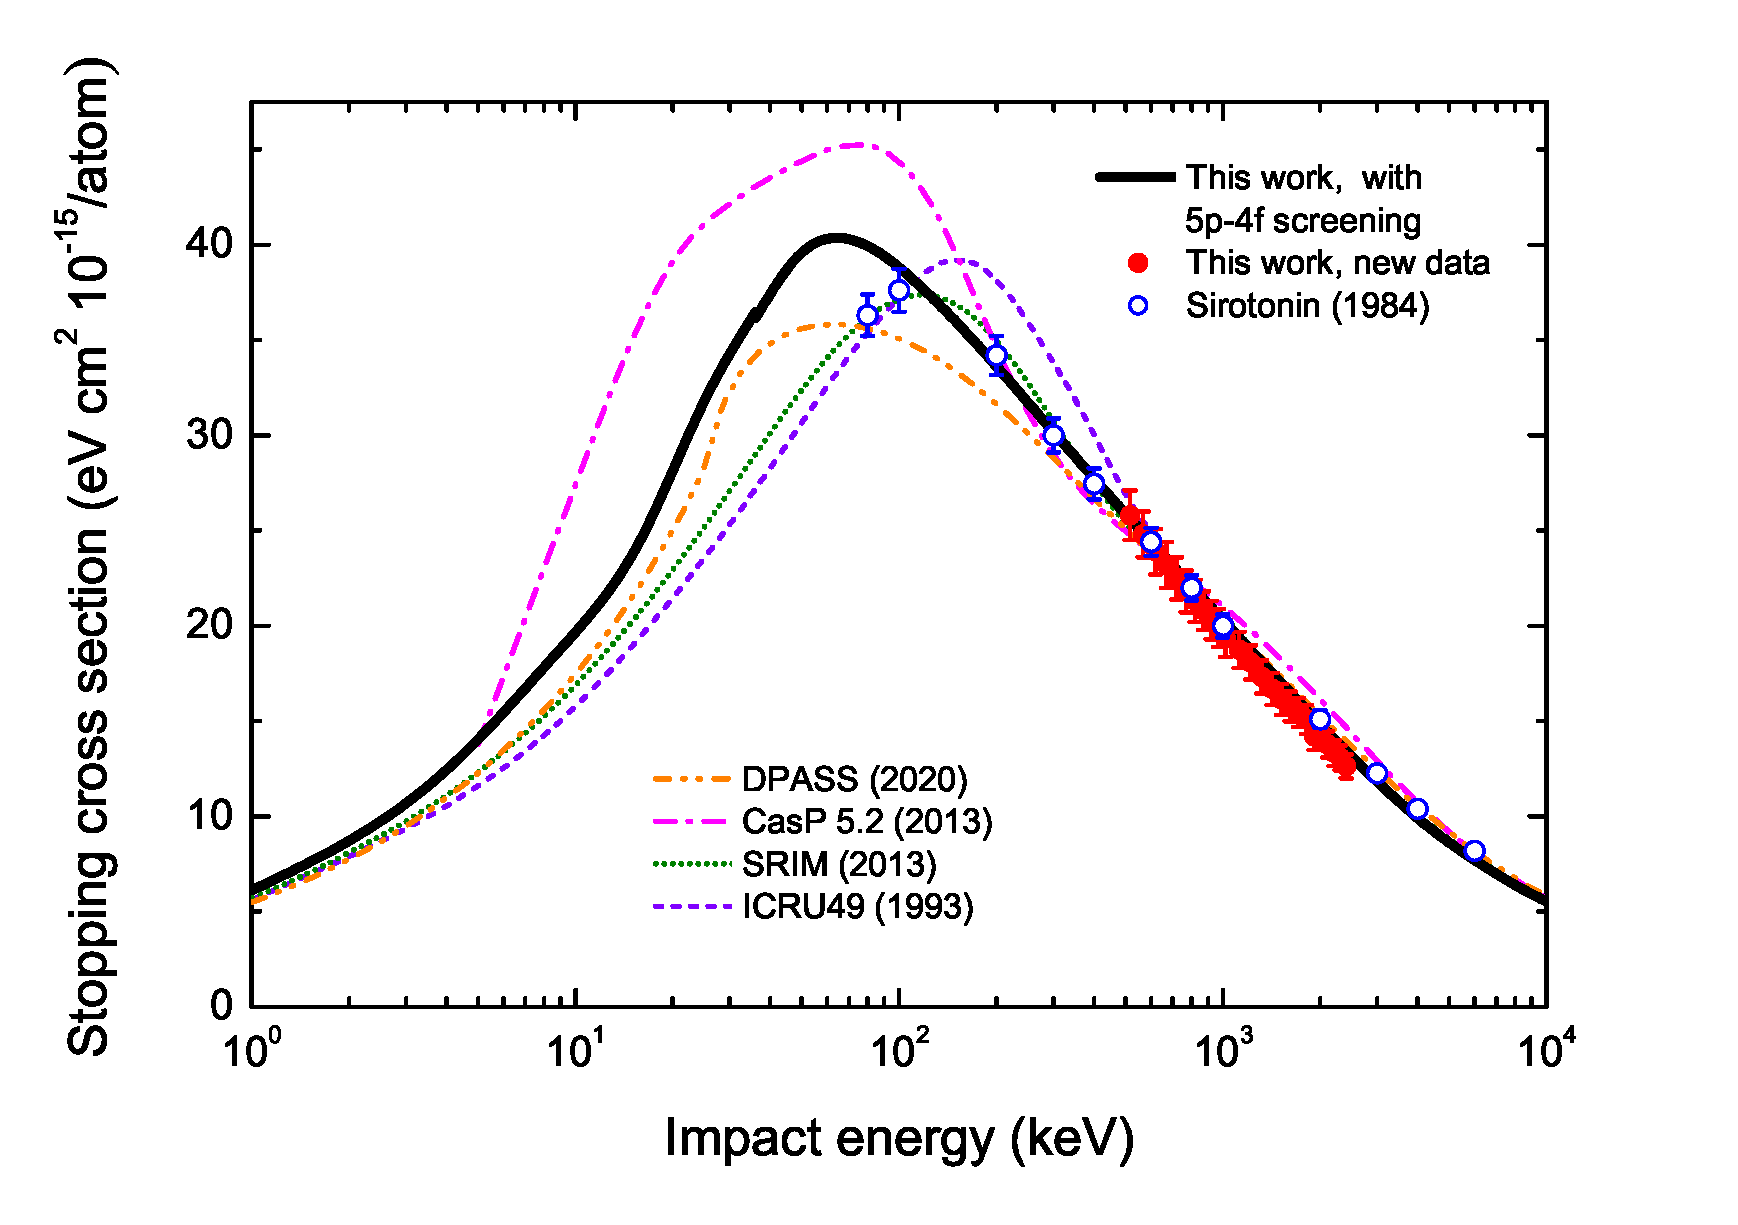
\includegraphics[width=13.0cm]{Fig03_new2.eps}
\caption{\DIFaddFL{(color online) Stopping power cross section of hafnium for 
protons. Symbols: solid circles, present values; open circles, previous 
data~\mbox{%DIFAUXCMD
\cite{Sirotinin}}\hspace{0pt}%DIFAUXCMD
. Curves: 
Black solid-line, present full theoretical results with $4f$-$5p$ screening; 
pink dash-dot line, theoretical CasP5.2~\mbox{%DIFAUXCMD
\cite{Grande,casp52} }\hspace{0pt}%DIFAUXCMD
values; 
orange dash-double-dot line, theoretical DPASS~\mbox{%DIFAUXCMD
\cite{DPASS20} }\hspace{0pt}%DIFAUXCMD
results; 
green dotted-line, semi-empirical SRIM-2013~\mbox{%DIFAUXCMD
\cite{Ziegler01}}\hspace{0pt}%DIFAUXCMD
; 
violet dashed-line, ICRU49~\mbox{%DIFAUXCMD
\cite{ICRU49} }\hspace{0pt}%DIFAUXCMD
tabulated values.}}
\DIFaddendFL \label{F03}
\end{figure*}
%DIF < =============================================================================================================================================================================================
%DIF > -----------------------------------------------------------------------

In Fig.~\ref{slpa4f}, we display the present theoretical stopping cross
section of Hf for protons \DIFaddbegin \DIFadd{using the relativistic wave functions 
and binding energies, but }\DIFaddend with and without the $5p$-$4f$ screening. 
We \DIFdelbegin \DIFdel{added }\DIFdelend \DIFaddbegin \DIFadd{show }\DIFaddend the FEG and \DIFdelbegin \DIFdel{the }\DIFdelend bound electron contributions \DIFdelbegin \DIFdel{as explained above}\DIFdelend \DIFaddbegin \DIFadd{separately and the 
total stopping as the addition of both of them}\DIFaddend . The minimum energy for 
plasmon excitation was estimated \DIFdelbegin \DIFdel{to }\DIFdelend \DIFaddbegin \DIFadd{at approximately }\DIFaddend $37$ keV. We used the 
non-perturbative SPCC model for impact energies $E \leq 37$\DIFaddbegin \DIFadd{~}\DIFaddend keV, and the 
perturbative ML calculation above this \DIFdelbegin \DIFdel{energy. %DIF < The range of validity of the perturbative model below 100 keV is arguable, however the asymetric $Z_{ion}/Z_{target}$ relation is clear. 
%DIF < The importance of the 4f-5p screening is signed with arrows in this figure. 
Clearly, considering }\DIFdelend \DIFaddbegin \DIFadd{value. Bound $1s$-$4f$ electrons 
(relativistic wave functions and binding energies) are calculated with 
the SLPA and shown separately in Fig.~\ref{slpa4f} with and without the 
$4f$-$5p$ screening. Below $\sim 40$ keV, the difference between both 
calculations is negligible. Considering }\DIFaddend $5p$-$4f$ electrons 
as a single group of 20 electrons with screening among them gives lower 
stopping values than the addition of the separate $5p$ and $4f$ 
contributions. Notice that this shell correction can \DIFdelbegin \DIFdel{only be considered 
within a many electron model}\DIFdelend \DIFaddbegin \DIFadd{be considered 
naturally within a many-electron model, }\DIFaddend such as the SLPA.

%DIF < =============================================================================================================================================================================================
%DIF > =======================================================================
\section{Analysis of the results and discussion}
\label{discussion}

The present data \DIFdelbegin \DIFdel{and theoretical results }\DIFdelend are displayed in Table~\ref{table01}\DIFdelbegin \DIFdel{, and Fig.~\ref{F03}}\DIFdelend . As can be 
\DIFdelbegin \DIFdel{seen in Table~\ref{table01}}\DIFdelend \DIFaddbegin \DIFadd{observed}\DIFaddend , an overall relative uncertainty 
of around 5\% was achieved for the experimental stopping power values, 
which are mainly due to the uncertainty in the hafnium foil thickness. 

%DIF < -----------------TABLE--------------------------------------------------------------------------
%DIF > -----------------------------------------------------------------------
\begin{table*}[!t]
\centering
\caption{Stopping power values S\DIFdelbeginFL \DIFdelFL{$_{exp}$ }\DIFdelendFL \DIFaddbeginFL \DIFaddFL{$_{\mathrm{exp}}$ }\DIFaddendFL of hafnium for protons 
measured in this work. $\Delta$E/E values are also shown.\DIFdelbeginFL %DIFDELCMD < \label{table01}%%%
\DIFdelendFL }
\DIFaddbeginFL \label{table01}
\DIFaddendFL 

\vspace{0.2cm}

\begin{ruledtabular}
\begin{tabular}{ccc|ccc|ccc} %\hline\hline
E\DIFdelbeginFL \DIFdelFL{$_{avg}$	}\DIFdelendFL \DIFaddbeginFL \DIFaddFL{$_{\mathrm{avg}}$ }\DIFaddendFL & S\DIFdelbeginFL \DIFdelFL{$_{exp}$			}\DIFdelendFL \DIFaddbeginFL \DIFaddFL{$_{\mathrm{exp}}$       }\DIFaddendFL & $\Delta$E/E & E\DIFdelbeginFL \DIFdelFL{$_{avg}$	}\DIFdelendFL \DIFaddbeginFL \DIFaddFL{$_{\mathrm{avg}}$ }\DIFaddendFL & S\DIFdelbeginFL \DIFdelFL{$_{exp}$			}\DIFdelendFL \DIFaddbeginFL \DIFaddFL{$_{\mathrm{exp}}$       }\DIFaddendFL & $\Delta$E/E & E\DIFdelbeginFL \DIFdelFL{$_{avg}$	}\DIFdelendFL \DIFaddbeginFL \DIFaddFL{$_{\mathrm{avg}}$ }\DIFaddendFL & S\DIFdelbeginFL \DIFdelFL{$_{exp}$			}\DIFdelendFL \DIFaddbeginFL \DIFaddFL{$_{\mathrm{exp}}$       }\DIFaddendFL & $\Delta$E/E \\
keV                & eV/(10$^{15}$ at/cm$^2$) & \DIFdelbeginFL \DIFdelFL{$\%$		}\DIFdelendFL \DIFaddbeginFL \DIFaddFL{\%          }\DIFaddendFL & keV                & eV/(10$^{15}$ at/cm$^2$)	& \DIFdelbeginFL \DIFdelFL{$\%$		}\DIFdelendFL \DIFaddbeginFL \DIFaddFL{\%          }\DIFaddendFL & keV                & eV/(10$^{15}$ at/cm$^2$) & \DIFdelbeginFL \DIFdelFL{$\%$}\DIFdelendFL \DIFaddbeginFL \DIFaddFL{\% }\DIFaddendFL \\ \hline
\DIFdelbeginFL \DIFdelFL{516,6	}\DIFdelendFL \DIFaddbeginFL \DIFaddFL{516.6	 }\DIFaddendFL & \DIFdelbeginFL \DIFdelFL{25,8	}\DIFdelendFL \DIFaddbeginFL \DIFaddFL{25.8	}\DIFaddendFL $\pm$	\DIFdelbeginFL \DIFdelFL{1,3	}\DIFdelendFL \DIFaddbeginFL \DIFaddFL{1.3	}\DIFaddendFL &	\DIFdelbeginFL \DIFdelFL{20,5	}\DIFdelendFL \DIFaddbeginFL \DIFaddFL{20.5	}\DIFaddendFL &	\DIFdelbeginFL \DIFdelFL{1170,3	}\DIFdelendFL \DIFaddbeginFL \DIFaddFL{1170.3	}\DIFaddendFL &	\DIFdelbeginFL \DIFdelFL{18,25	}\DIFdelendFL \DIFaddbeginFL \DIFaddFL{18.25	}\DIFaddendFL $\pm$	\DIFdelbeginFL \DIFdelFL{0,91	}\DIFdelendFL \DIFaddbeginFL \DIFaddFL{0.91	}\DIFaddendFL &	\DIFdelbeginFL \DIFdelFL{6,4	}\DIFdelendFL \DIFaddbeginFL \DIFaddFL{6.4	}\DIFaddendFL &	\DIFdelbeginFL \DIFdelFL{1813,4	}\DIFdelendFL \DIFaddbeginFL \DIFaddFL{1813.4	}\DIFaddendFL &	\DIFdelbeginFL \DIFdelFL{15,10	}\DIFdelendFL \DIFaddbeginFL \DIFaddFL{15.10	}\DIFaddendFL $\pm$	\DIFdelbeginFL \DIFdelFL{0,76	}\DIFdelendFL \DIFaddbeginFL \DIFaddFL{0.76	}\DIFaddendFL &	\DIFdelbeginFL \DIFdelFL{3,4	}\DIFdelendFL \DIFaddbeginFL \DIFaddFL{3.4	}\DIFaddendFL \\
\DIFdelbeginFL \DIFdelFL{567,8	}\DIFdelendFL \DIFaddbeginFL \DIFaddFL{567.8	 }\DIFaddendFL & \DIFdelbeginFL \DIFdelFL{24,8	}\DIFdelendFL \DIFaddbeginFL \DIFaddFL{24.8	}\DIFaddendFL $\pm$	\DIFdelbeginFL \DIFdelFL{1,2	}\DIFdelendFL \DIFaddbeginFL \DIFaddFL{1.2	}\DIFaddendFL &	\DIFdelbeginFL \DIFdelFL{17,9	}\DIFdelendFL \DIFaddbeginFL \DIFaddFL{17.9	}\DIFaddendFL &	\DIFdelbeginFL \DIFdelFL{1220,0	}\DIFdelendFL \DIFaddbeginFL \DIFaddFL{1220.0	}\DIFaddendFL &	\DIFdelbeginFL \DIFdelFL{18,08	}\DIFdelendFL \DIFaddbeginFL \DIFaddFL{18.08	}\DIFaddendFL $\pm$	\DIFdelbeginFL \DIFdelFL{0,90	}\DIFdelendFL \DIFaddbeginFL \DIFaddFL{0.90	}\DIFaddendFL &	\DIFdelbeginFL \DIFdelFL{6,1	}\DIFdelendFL \DIFaddbeginFL \DIFaddFL{6.1	}\DIFaddendFL &	\DIFdelbeginFL \DIFdelFL{1862,7	}\DIFdelendFL \DIFaddbeginFL \DIFaddFL{1862.7	}\DIFaddendFL &	\DIFdelbeginFL \DIFdelFL{14,79	}\DIFdelendFL \DIFaddbeginFL \DIFaddFL{14.79	}\DIFaddendFL $\pm$	\DIFdelbeginFL \DIFdelFL{0,74	}\DIFdelendFL \DIFaddbeginFL \DIFaddFL{0.74	}\DIFaddendFL &	\DIFdelbeginFL \DIFdelFL{3,3	}\DIFdelendFL \DIFaddbeginFL \DIFaddFL{3.3	}\DIFaddendFL \\
\DIFdelbeginFL \DIFdelFL{618,8	}\DIFdelendFL \DIFaddbeginFL \DIFaddFL{618.8	 }\DIFaddendFL & \DIFdelbeginFL \DIFdelFL{23,9	}\DIFdelendFL \DIFaddbeginFL \DIFaddFL{23.9	}\DIFaddendFL $\pm$	\DIFdelbeginFL \DIFdelFL{1,2	}\DIFdelendFL \DIFaddbeginFL \DIFaddFL{1.2	}\DIFaddendFL &	\DIFdelbeginFL \DIFdelFL{15,8	}\DIFdelendFL \DIFaddbeginFL \DIFaddFL{15.8	}\DIFaddendFL &	\DIFdelbeginFL \DIFdelFL{1269,6	}\DIFdelendFL \DIFaddbeginFL \DIFaddFL{1269.6	}\DIFaddendFL &	\DIFdelbeginFL \DIFdelFL{17,57	}\DIFdelendFL \DIFaddbeginFL \DIFaddFL{17.57	}\DIFaddendFL $\pm$	\DIFdelbeginFL \DIFdelFL{0,88	}\DIFdelendFL \DIFaddbeginFL \DIFaddFL{0.88	}\DIFaddendFL &	\DIFdelbeginFL \DIFdelFL{5,7	}\DIFdelendFL \DIFaddbeginFL \DIFaddFL{5.7	}\DIFaddendFL &	\DIFdelbeginFL \DIFdelFL{1912,0	}\DIFdelendFL \DIFaddbeginFL \DIFaddFL{1912.0	}\DIFaddendFL &	\DIFdelbeginFL \DIFdelFL{14,21	}\DIFdelendFL \DIFaddbeginFL \DIFaddFL{14.21	}\DIFaddendFL $\pm$	\DIFdelbeginFL \DIFdelFL{0,71	}\DIFdelendFL \DIFaddbeginFL \DIFaddFL{0.71	}\DIFaddendFL &	\DIFdelbeginFL \DIFdelFL{3,0	}\DIFdelendFL \DIFaddbeginFL \DIFaddFL{3.0	}\DIFaddendFL \\
\DIFdelbeginFL \DIFdelFL{669,6	}\DIFdelendFL \DIFaddbeginFL \DIFaddFL{669.6	 }\DIFaddendFL & \DIFdelbeginFL \DIFdelFL{23,2	}\DIFdelendFL \DIFaddbeginFL \DIFaddFL{23.2	}\DIFaddendFL $\pm$	\DIFdelbeginFL \DIFdelFL{1,2	}\DIFdelendFL \DIFaddbeginFL \DIFaddFL{1.2	}\DIFaddendFL &	\DIFdelbeginFL \DIFdelFL{14,2	}\DIFdelendFL \DIFaddbeginFL \DIFaddFL{14.2	}\DIFaddendFL &	\DIFdelbeginFL \DIFdelFL{1319,2	}\DIFdelendFL \DIFaddbeginFL \DIFaddFL{1319.2	}\DIFaddendFL &	\DIFdelbeginFL \DIFdelFL{17,32	}\DIFdelendFL \DIFaddbeginFL \DIFaddFL{17.32	}\DIFaddendFL $\pm$	\DIFdelbeginFL \DIFdelFL{0,87	}\DIFdelendFL \DIFaddbeginFL \DIFaddFL{0.87	}\DIFaddendFL &	\DIFdelbeginFL \DIFdelFL{5,4	}\DIFdelendFL \DIFaddbeginFL \DIFaddFL{5.4	}\DIFaddendFL &	\DIFdelbeginFL \DIFdelFL{1961,2	}\DIFdelendFL \DIFaddbeginFL \DIFaddFL{1961.2	}\DIFaddendFL &	\DIFdelbeginFL \DIFdelFL{14,46	}\DIFdelendFL \DIFaddbeginFL \DIFaddFL{14.46	}\DIFaddendFL $\pm$	\DIFdelbeginFL \DIFdelFL{0,72	}\DIFdelendFL \DIFaddbeginFL \DIFaddFL{0.72	}\DIFaddendFL &	\DIFdelbeginFL \DIFdelFL{3,0	}\DIFdelendFL \DIFaddbeginFL \DIFaddFL{3.0	}\DIFaddendFL \\
\DIFdelbeginFL \DIFdelFL{720,1	}\DIFdelendFL \DIFaddbeginFL \DIFaddFL{720.1	 }\DIFaddendFL & \DIFdelbeginFL \DIFdelFL{22,5	}\DIFdelendFL \DIFaddbeginFL \DIFaddFL{22.5	}\DIFaddendFL $\pm$	\DIFdelbeginFL \DIFdelFL{1,1	}\DIFdelendFL \DIFaddbeginFL \DIFaddFL{1.1	}\DIFaddendFL &	\DIFdelbeginFL \DIFdelFL{12,8	}\DIFdelendFL \DIFaddbeginFL \DIFaddFL{12.8	}\DIFaddendFL &	\DIFdelbeginFL \DIFdelFL{1368,8	}\DIFdelendFL \DIFaddbeginFL \DIFaddFL{1368.8	}\DIFaddendFL &	\DIFdelbeginFL \DIFdelFL{17,15	}\DIFdelendFL \DIFaddbeginFL \DIFaddFL{17.15	}\DIFaddendFL $\pm$	\DIFdelbeginFL \DIFdelFL{0,86	}\DIFdelendFL \DIFaddbeginFL \DIFaddFL{0.86	}\DIFaddendFL &	\DIFdelbeginFL \DIFdelFL{5,1	}\DIFdelendFL \DIFaddbeginFL \DIFaddFL{5.1	}\DIFaddendFL &	\DIFdelbeginFL \DIFdelFL{2010,4	}\DIFdelendFL \DIFaddbeginFL \DIFaddFL{2010.4	}\DIFaddendFL &	\DIFdelbeginFL \DIFdelFL{14,34	}\DIFdelendFL \DIFaddbeginFL \DIFaddFL{14.34	}\DIFaddendFL $\pm$	\DIFdelbeginFL \DIFdelFL{0,72	}\DIFdelendFL \DIFaddbeginFL \DIFaddFL{0.72	}\DIFaddendFL &	\DIFdelbeginFL \DIFdelFL{2,9	}\DIFdelendFL \DIFaddbeginFL \DIFaddFL{2.9	}\DIFaddendFL \\
\DIFdelbeginFL \DIFdelFL{770,5	}\DIFdelendFL \DIFaddbeginFL \DIFaddFL{770.5	 }\DIFaddendFL & \DIFdelbeginFL \DIFdelFL{21,8	}\DIFdelendFL \DIFaddbeginFL \DIFaddFL{21.8	}\DIFaddendFL $\pm$	\DIFdelbeginFL \DIFdelFL{1,1	}\DIFdelendFL \DIFaddbeginFL \DIFaddFL{1.1	}\DIFaddendFL &	\DIFdelbeginFL \DIFdelFL{11,6	}\DIFdelendFL \DIFaddbeginFL \DIFaddFL{11.6	}\DIFaddendFL &	\DIFdelbeginFL \DIFdelFL{1418,3	}\DIFdelendFL \DIFaddbeginFL \DIFaddFL{1418.3	}\DIFaddendFL &	\DIFdelbeginFL \DIFdelFL{16,69	}\DIFdelendFL \DIFaddbeginFL \DIFaddFL{16.69	}\DIFaddendFL $\pm$	\DIFdelbeginFL \DIFdelFL{0,83	}\DIFdelendFL \DIFaddbeginFL \DIFaddFL{0.83	}\DIFaddendFL &	\DIFdelbeginFL \DIFdelFL{4,8	}\DIFdelendFL \DIFaddbeginFL \DIFaddFL{4.8	}\DIFaddendFL &	\DIFdelbeginFL \DIFdelFL{2059,6	}\DIFdelendFL \DIFaddbeginFL \DIFaddFL{2059.6	}\DIFaddendFL &	\DIFdelbeginFL \DIFdelFL{13,76	}\DIFdelendFL \DIFaddbeginFL \DIFaddFL{13.76	}\DIFaddendFL $\pm$	\DIFdelbeginFL \DIFdelFL{0,69	}\DIFdelendFL \DIFaddbeginFL \DIFaddFL{0.69	}\DIFaddendFL &	\DIFdelbeginFL \DIFdelFL{2,7	}\DIFdelendFL \DIFaddbeginFL \DIFaddFL{2.7	}\DIFaddendFL \\
\DIFdelbeginFL \DIFdelFL{820,8	}\DIFdelendFL \DIFaddbeginFL \DIFaddFL{820.8	 }\DIFaddendFL & \DIFdelbeginFL \DIFdelFL{21,3	}\DIFdelendFL \DIFaddbeginFL \DIFaddFL{21.3	}\DIFaddendFL $\pm$	\DIFdelbeginFL \DIFdelFL{1,1	}\DIFdelendFL \DIFaddbeginFL \DIFaddFL{1.1	}\DIFaddendFL &	\DIFdelbeginFL \DIFdelFL{10,7	}\DIFdelendFL \DIFaddbeginFL \DIFaddFL{10.7	}\DIFaddendFL &	\DIFdelbeginFL \DIFdelFL{1467,8	}\DIFdelendFL \DIFaddbeginFL \DIFaddFL{1467.8	}\DIFaddendFL &	\DIFdelbeginFL \DIFdelFL{16,43	}\DIFdelendFL \DIFaddbeginFL \DIFaddFL{16.43	}\DIFaddendFL $\pm$	\DIFdelbeginFL \DIFdelFL{0,82	}\DIFdelendFL \DIFaddbeginFL \DIFaddFL{0.82	}\DIFaddendFL &	\DIFdelbeginFL \DIFdelFL{4,6	}\DIFdelendFL \DIFaddbeginFL \DIFaddFL{4.6	}\DIFaddendFL &	\DIFdelbeginFL \DIFdelFL{2108,8	}\DIFdelendFL \DIFaddbeginFL \DIFaddFL{2108.8	}\DIFaddendFL &	\DIFdelbeginFL \DIFdelFL{13,78	}\DIFdelendFL \DIFaddbeginFL \DIFaddFL{13.78	}\DIFaddendFL $\pm$	\DIFdelbeginFL \DIFdelFL{0,69	}\DIFdelendFL \DIFaddbeginFL \DIFaddFL{0.69	}\DIFaddendFL &	\DIFdelbeginFL \DIFdelFL{2,7	}\DIFdelendFL \DIFaddbeginFL \DIFaddFL{2.7	}\DIFaddendFL \\
\DIFdelbeginFL \DIFdelFL{871,0	}\DIFdelendFL \DIFaddbeginFL \DIFaddFL{871.0	 }\DIFaddendFL & \DIFdelbeginFL \DIFdelFL{20,8	}\DIFdelendFL \DIFaddbeginFL \DIFaddFL{20.8	}\DIFaddendFL $\pm$	\DIFdelbeginFL \DIFdelFL{1,0	}\DIFdelendFL \DIFaddbeginFL \DIFaddFL{1.0	}\DIFaddendFL &	\DIFdelbeginFL \DIFdelFL{9,8	}\DIFdelendFL \DIFaddbeginFL \DIFaddFL{9.8	}\DIFaddendFL &	\DIFdelbeginFL \DIFdelFL{1517,2	}\DIFdelendFL \DIFaddbeginFL \DIFaddFL{1517.2	}\DIFaddendFL &	\DIFdelbeginFL \DIFdelFL{16,13	}\DIFdelendFL \DIFaddbeginFL \DIFaddFL{16.13	}\DIFaddendFL $\pm$	\DIFdelbeginFL \DIFdelFL{0,81	}\DIFdelendFL \DIFaddbeginFL \DIFaddFL{0.81	}\DIFaddendFL &	\DIFdelbeginFL \DIFdelFL{4,4	}\DIFdelendFL \DIFaddbeginFL \DIFaddFL{4.4	}\DIFaddendFL &	\DIFdelbeginFL \DIFdelFL{2158,0	}\DIFdelendFL \DIFaddbeginFL \DIFaddFL{2158.0	}\DIFaddendFL &	\DIFdelbeginFL \DIFdelFL{13,70	}\DIFdelendFL \DIFaddbeginFL \DIFaddFL{13.70	}\DIFaddendFL $\pm$	\DIFdelbeginFL \DIFdelFL{0,69	}\DIFdelendFL \DIFaddbeginFL \DIFaddFL{0.69	}\DIFaddendFL &	\DIFdelbeginFL \DIFdelFL{2,6	}\DIFdelendFL \DIFaddbeginFL \DIFaddFL{2.6	}\DIFaddendFL \\
\DIFdelbeginFL \DIFdelFL{921,1	}\DIFdelendFL \DIFaddbeginFL \DIFaddFL{921.1	 }\DIFaddendFL & \DIFdelbeginFL \DIFdelFL{20,3	}\DIFdelendFL \DIFaddbeginFL \DIFaddFL{20.3	}\DIFaddendFL $\pm$	\DIFdelbeginFL \DIFdelFL{1,0	}\DIFdelendFL \DIFaddbeginFL \DIFaddFL{1.0	}\DIFaddendFL &	\DIFdelbeginFL \DIFdelFL{9,1	}\DIFdelendFL \DIFaddbeginFL \DIFaddFL{9.1	}\DIFaddendFL &	\DIFdelbeginFL \DIFdelFL{1566,7	}\DIFdelendFL \DIFaddbeginFL \DIFaddFL{1566.7	}\DIFaddendFL &	\DIFdelbeginFL \DIFdelFL{16,04	}\DIFdelendFL \DIFaddbeginFL \DIFaddFL{16.04	}\DIFaddendFL $\pm$	\DIFdelbeginFL \DIFdelFL{0,80	}\DIFdelendFL \DIFaddbeginFL \DIFaddFL{0.80	}\DIFaddendFL &	\DIFdelbeginFL \DIFdelFL{4,2	}\DIFdelendFL \DIFaddbeginFL \DIFaddFL{4.2	}\DIFaddendFL &	\DIFdelbeginFL \DIFdelFL{2206,5	}\DIFdelendFL \DIFaddbeginFL \DIFaddFL{2206.5	}\DIFaddendFL &	\DIFdelbeginFL \DIFdelFL{13,33	}\DIFdelendFL \DIFaddbeginFL \DIFaddFL{13.33	}\DIFaddendFL $\pm$	\DIFdelbeginFL \DIFdelFL{0,67	}\DIFdelendFL \DIFaddbeginFL \DIFaddFL{0.67	}\DIFaddendFL &	\DIFdelbeginFL \DIFdelFL{2,5	}\DIFdelendFL \DIFaddbeginFL \DIFaddFL{2.5	}\DIFaddendFL \\
\DIFdelbeginFL \DIFdelFL{971,1	}\DIFdelendFL \DIFaddbeginFL \DIFaddFL{971.1	 }\DIFaddendFL & \DIFdelbeginFL \DIFdelFL{19,9	}\DIFdelendFL \DIFaddbeginFL \DIFaddFL{19.9	}\DIFaddendFL $\pm$	\DIFdelbeginFL \DIFdelFL{1,0	}\DIFdelendFL \DIFaddbeginFL \DIFaddFL{1.0	}\DIFaddendFL &	\DIFdelbeginFL \DIFdelFL{8,4	}\DIFdelendFL \DIFaddbeginFL \DIFaddFL{8.4	}\DIFaddendFL &	\DIFdelbeginFL \DIFdelFL{1616,0	}\DIFdelendFL \DIFaddbeginFL \DIFaddFL{1616.0	}\DIFaddendFL &	\DIFdelbeginFL \DIFdelFL{15,77	}\DIFdelendFL \DIFaddbeginFL \DIFaddFL{15.77	}\DIFaddendFL $\pm$	\DIFdelbeginFL \DIFdelFL{0,79	}\DIFdelendFL \DIFaddbeginFL \DIFaddFL{0.79	}\DIFaddendFL &	\DIFdelbeginFL \DIFdelFL{4,0	}\DIFdelendFL \DIFaddbeginFL \DIFaddFL{4.0	}\DIFaddendFL &	\DIFdelbeginFL \DIFdelFL{2256,4	}\DIFdelendFL \DIFaddbeginFL \DIFaddFL{2256.4	}\DIFaddendFL &	\DIFdelbeginFL \DIFdelFL{13,27	}\DIFdelendFL \DIFaddbeginFL \DIFaddFL{13.27	}\DIFaddendFL $\pm$	\DIFdelbeginFL \DIFdelFL{0,66	}\DIFdelendFL \DIFaddbeginFL \DIFaddFL{0.66	}\DIFaddendFL &	\DIFdelbeginFL \DIFdelFL{2,4	}\DIFdelendFL \DIFaddbeginFL \DIFaddFL{2.4	}\DIFaddendFL \\
\DIFdelbeginFL \DIFdelFL{1021,0	}\DIFdelendFL \DIFaddbeginFL \DIFaddFL{1021.0 }\DIFaddendFL & \DIFdelbeginFL \DIFdelFL{19,33	}\DIFdelendFL \DIFaddbeginFL \DIFaddFL{19.33	}\DIFaddendFL $\pm$	\DIFdelbeginFL \DIFdelFL{0,97	}\DIFdelendFL \DIFaddbeginFL \DIFaddFL{0.97	}\DIFaddendFL &	\DIFdelbeginFL \DIFdelFL{7,8	}\DIFdelendFL \DIFaddbeginFL \DIFaddFL{7.8	}\DIFaddendFL &	\DIFdelbeginFL \DIFdelFL{1665,4	}\DIFdelendFL \DIFaddbeginFL \DIFaddFL{1665.4	}\DIFaddendFL &	\DIFdelbeginFL \DIFdelFL{15,51	}\DIFdelendFL \DIFaddbeginFL \DIFaddFL{15.51	}\DIFaddendFL $\pm$	\DIFdelbeginFL \DIFdelFL{0,78	}\DIFdelendFL \DIFaddbeginFL \DIFaddFL{0.78	}\DIFaddendFL &	\DIFdelbeginFL \DIFdelFL{3,8	}\DIFdelendFL \DIFaddbeginFL \DIFaddFL{3.8	}\DIFaddendFL &	\DIFdelbeginFL \DIFdelFL{2305,5	}\DIFdelendFL \DIFaddbeginFL \DIFaddFL{2305.5	}\DIFaddendFL &	\DIFdelbeginFL \DIFdelFL{13,07	}\DIFdelendFL \DIFaddbeginFL \DIFaddFL{13.07	}\DIFaddendFL $\pm$	\DIFdelbeginFL \DIFdelFL{0,65	}\DIFdelendFL \DIFaddbeginFL \DIFaddFL{0.65	}\DIFaddendFL &	\DIFdelbeginFL \DIFdelFL{2,3	}\DIFdelendFL \DIFaddbeginFL \DIFaddFL{2.3	}\DIFaddendFL \\
\DIFdelbeginFL \DIFdelFL{1070,8	}\DIFdelendFL \DIFaddbeginFL \DIFaddFL{1070.8 }\DIFaddendFL & \DIFdelbeginFL \DIFdelFL{19,03	}\DIFdelendFL \DIFaddbeginFL \DIFaddFL{19.03	}\DIFaddendFL $\pm$	\DIFdelbeginFL \DIFdelFL{0,95	}\DIFdelendFL \DIFaddbeginFL \DIFaddFL{0.95	}\DIFaddendFL &	\DIFdelbeginFL \DIFdelFL{7,3	}\DIFdelendFL \DIFaddbeginFL \DIFaddFL{7.3	}\DIFaddendFL &	\DIFdelbeginFL \DIFdelFL{1714,8	}\DIFdelendFL \DIFaddbeginFL \DIFaddFL{1714.8	}\DIFaddendFL &	\DIFdelbeginFL \DIFdelFL{15,46	}\DIFdelendFL \DIFaddbeginFL \DIFaddFL{15.46	}\DIFaddendFL $\pm$	\DIFdelbeginFL \DIFdelFL{0,77	}\DIFdelendFL \DIFaddbeginFL \DIFaddFL{0.77	}\DIFaddendFL &	\DIFdelbeginFL \DIFdelFL{3,7	}\DIFdelendFL \DIFaddbeginFL \DIFaddFL{3.7	}\DIFaddendFL &	\DIFdelbeginFL \DIFdelFL{2354,7	}\DIFdelendFL \DIFaddbeginFL \DIFaddFL{2354.7	}\DIFaddendFL &	\DIFdelbeginFL \DIFdelFL{12,91	}\DIFdelendFL \DIFaddbeginFL \DIFaddFL{12.91	}\DIFaddendFL $\pm$	\DIFdelbeginFL \DIFdelFL{0,65	}\DIFdelendFL \DIFaddbeginFL \DIFaddFL{0.65	}\DIFaddendFL &	\DIFdelbeginFL \DIFdelFL{2,2	}\DIFdelendFL \DIFaddbeginFL \DIFaddFL{2.2	}\DIFaddendFL \\
\DIFdelbeginFL \DIFdelFL{1120,6	}\DIFdelendFL \DIFaddbeginFL \DIFaddFL{1120.6 }\DIFaddendFL & \DIFdelbeginFL \DIFdelFL{18,73	}\DIFdelendFL \DIFaddbeginFL \DIFaddFL{18.73	}\DIFaddendFL $\pm$	\DIFdelbeginFL \DIFdelFL{0,94	}\DIFdelendFL \DIFaddbeginFL \DIFaddFL{0.94	}\DIFaddendFL &	\DIFdelbeginFL \DIFdelFL{6,9	}\DIFdelendFL \DIFaddbeginFL \DIFaddFL{6.9	}\DIFaddendFL &	\DIFdelbeginFL \DIFdelFL{1764,1	}\DIFdelendFL \DIFaddbeginFL \DIFaddFL{1764.1	}\DIFaddendFL &	\DIFdelbeginFL \DIFdelFL{14,93	}\DIFdelendFL \DIFaddbeginFL \DIFaddFL{14.93	}\DIFaddendFL $\pm$	\DIFdelbeginFL \DIFdelFL{0,75	}\DIFdelendFL \DIFaddbeginFL \DIFaddFL{0.75	}\DIFaddendFL &	\DIFdelbeginFL \DIFdelFL{3,5	}\DIFdelendFL \DIFaddbeginFL \DIFaddFL{3.5	}\DIFaddendFL &	\DIFdelbeginFL \DIFdelFL{2403,8	}\DIFdelendFL \DIFaddbeginFL \DIFaddFL{2403.8	}\DIFaddendFL &	\DIFdelbeginFL \DIFdelFL{12,61	}\DIFdelendFL \DIFaddbeginFL \DIFaddFL{12.61	}\DIFaddendFL $\pm$	\DIFdelbeginFL \DIFdelFL{0,63	}\DIFdelendFL \DIFaddbeginFL \DIFaddFL{0.63	}\DIFaddendFL &	\DIFdelbeginFL \DIFdelFL{2,2	}\DIFdelendFL \DIFaddbeginFL \DIFaddFL{2.2	}\DIFaddendFL \\ \\ 
%DIF < \hline
\end{tabular}
\end{ruledtabular}
\end{table*}

\DIFdelbegin \DIFdel{In }\DIFdelend Fig.~\ref{F03} \DIFdelbegin \DIFdel{, we have good }\DIFdelend \DIFaddbegin \DIFadd{synthesizes the results of the present work. The 
}\DIFaddend agreement between the present theoretical results and the \DIFaddbegin \DIFadd{new 
}\DIFaddend measurements displayed in Table~\ref{table01} \DIFaddbegin \DIFadd{is excellent. Present 
measurements using the transmission method are in good agreement with 
the previous data by Sirotinin~\mbox{%DIFAUXCMD
\cite{Sirotinin}}\hspace{0pt}%DIFAUXCMD
, which were measured 
in backscattering geometry}\DIFaddend . Our theoretical approach also agrees with 
\DIFdelbegin \DIFdel{previous }\DIFdelend \DIFaddbegin \DIFadd{the }\DIFaddend data by Sirotinin~\cite{Sirotinin}, except for the lowest energy 
measurement at 80 keV. \DIFdelbegin \DIFdel{It is interesting that }\DIFdelend \DIFaddbegin \DIFadd{We have also included in this figure the 
theoretical curves from the CasP5.2 code by Grande and 
Schiwietz~\mbox{%DIFAUXCMD
\cite{Grande,casp52} }\hspace{0pt}%DIFAUXCMD
and from the DPASS code by Sigmund and 
Schinner~\mbox{%DIFAUXCMD
\cite{DPASS20}}\hspace{0pt}%DIFAUXCMD
, both available online. Furthermore, we 
incorporated the semi-empirical results from SRIM-2013~\mbox{%DIFAUXCMD
\cite{Ziegler01} 
}\hspace{0pt}%DIFAUXCMD
and the ICRU49 tables~\mbox{%DIFAUXCMD
\cite{ICRU49}}\hspace{0pt}%DIFAUXCMD
. Interestingly, }\DIFaddend our full theoretical 
curve differs from SRIM-2013 for impact energies below 100 keV. We 
obtain a stopping maximum \DIFdelbegin \DIFdel{around $40 \times 10^{-15}$ }\DIFdelend \DIFaddbegin \DIFadd{of approximately 
$40\times 10^{-15}$ }\DIFaddend eV cm$^2$/atom at 65 keV. Instead, following the 
up-to-now only set of data \DIFdelbegin \DIFdel{~}\DIFdelend \cite{Sirotinin}, SRIM-2013 suggests a lower 
stopping maximum at \DIFaddbegin \DIFadd{an }\DIFaddend impact energy of 115 \DIFdelbegin \DIFdel{kev}\DIFdelend \DIFaddbegin \DIFadd{keV. The stopping maximum is 
a susceptible region for any full theoretical description without 
parameters, and this is quite visible in a linear-scale plot like 
Fig.~\ref{F03}. However, the impact energy for the maximum seems to 
agree between our curve and DPASS, although it is $10 \%$ below. 
Instead, CasP a maximum value of the stopping power $10 \%$ above our 
value and a completely different shape at lower energies}\DIFaddend . It is worth 
mentioning that \DIFdelbegin \DIFdel{similar theoretical }\DIFdelend \DIFaddbegin \DIFadd{our model gives similar }\DIFaddend results using the experimental 
\DIFaddbegin \DIFadd{value }\DIFaddend $r_S=2.07$ a.u. \DIFdelbegin \DIFdel{instead of the theoretical }\DIFdelend \DIFaddbegin \DIFadd{rather than the theoretical one }\DIFaddend $r_S=2.14$ a.u.\DIFdelbegin \DIFdel{give }\DIFdelend \DIFaddbegin \DIFadd{,
with }\DIFaddend the stopping maximum at the same impact energy but $4\%$ higher. 
\DIFaddbegin 

\DIFaddend Future experiments for impact energies below 100 keV would be \DIFdelbegin \DIFdel{important }\DIFdelend \DIFaddbegin \DIFadd{essential 
}\DIFaddend to complete this study \DIFaddbegin \DIFadd{on the stopping of Hf for protons. In the energy 
region $80-500$ keV, only the measurements by Sirotinin's 
group~\mbox{%DIFAUXCMD
\cite{Sirotinin} }\hspace{0pt}%DIFAUXCMD
from 1984 are available. SRIM-2013 includes these 
values in the code fitting, so it does not represent a test for this 
data. Undoubtedly, new measurements are needed in three specific 
energy regions: below 500 keV, around the stopping maximum 
(i.e., $50-200$ keV), and at low impact energies}\DIFaddend . 

%DIF < =============================================================================================================================================================================================
%DIF < =============================================================================================================================================================================================
%DIF > =======================================================================
\section{Conclusion}
\label{conclusion}
\DIFaddbegin 

\DIFaddend In this work, we have used the transmission method to experimentally 
determine stopping power cross section values for (0.6-2.5) MeV protons 
incident on self-supporting Hf foils with an overall uncertainty of 
around 5\%. Additionally, we calculated values extracted from the 
theoretical framework that involved the relativistic wave functions and 
binding energies of Hf \DIFdelbegin \DIFdel{, and considered 4 }\DIFdelend \DIFaddbegin \DIFadd{and considered four }\DIFaddend electrons per atom in the 
free electron gas. The shell-wise local plasma approximation was 
employed to describe the energy transferred to the bound $1s$-$4f$ 
electrons, and two different models for the FEG: the screened potential 
with cusp condition (SPCC model) for energies below that of the plasmon 
excitation, and the Mermin-Lindhard dielectric formalism, for energies 
around the stopping maximum and above. Present theoretical stopping 
cross sections cover an extensive energy range from 1 keV/\DIFdelbegin \DIFdel{amu-10 meV}\DIFdelend \DIFaddbegin \DIFadd{amu to 
10 MeV}\DIFaddend /amu.

At high impact energies, the new stopping  measurements are in good 
agreement with our theoretical results, with previous experimental data
and semi-empirical values by SRIM-2013 and ICRU-49.  However, we call 
the attention that around the stopping maximum and at lower impact 
energies\DIFaddbegin \DIFadd{, }\DIFaddend the difference between our full-theoretical results and SRIM 
is substantial. \DIFaddbegin \DIFadd{We compare our theoretical results with two other models 
given by the DPASS and CasP5.2 codes. Differences can be noted at 
intermediate to low impact energies, but they also support a stopping 
maximum at lower energy than SRIM predictions. 
}

\DIFaddend To the best of our knowledge, these are the first theoretical 
calculations of stopping in Hf \DIFdelbegin \DIFdel{taking into account the atomic relativistic effect}\DIFdelend \DIFaddbegin \DIFadd{to take into account relativistic effects 
in the atomic structure and screening among electrons in a consistent 
way, from very low to high impact energies}\DIFaddend . Future experiments for 
impact energies \DIFdelbegin \DIFdel{below 100 keV would be important to complete this study.
%DIF < =======================================================================================================================================
}\DIFdelend \DIFaddbegin \DIFadd{around the stopping maximum and in the low energy region 
would be essential to have a better understanding of the stopping of 
protons in hafnium.
}

%DIF > =======================================================================
\DIFaddend \begin{acknowledgments}
This work was funded by VRAC Grant Number L1-17 of Universidad 
Tecnol\'ogica Metropolitana, Chile; also by the Consejo Nacional de 
Investigaciones Cient\'ificas y T\'ecnicas (CONICET), the Agencia 
Nacional de Promoci\'on Cient\'ifica y Tecnol\'ogica (ANPCyT), and 
Universidad de Buenos Aires (UBA), from Argentina.

The authors gratefully acknowledge the invaluable contribution of F. 
Baptista from ITN/IST-UTL, Sacav\'{e}m, Portugal for his constant 
availability. 
\end{acknowledgments}
\DIFdelbegin %DIFDELCMD < 

%DIFDELCMD < %%%
%DIF < =======================================================================================================================================
\DIFdelend %DIF > =======================================================================
%  references
\begin{thebibliography}{00}
%DIF < ============================================================================================================================
%DIF > =======================================================================
%Fundamentals of Stopping Power and Energy Loss processes
\bibitem{Chu01} 
W.K. Chu, J.W. Mayer, \DIFaddbegin \DIFadd{and }\DIFaddend M.A. Nicolet\DIFdelbegin \DIFdel{(Eds.) Backscattering Spectrometry,
}\DIFdelend \DIFaddbegin \DIFadd{,
}\textit{\DIFadd{Backscattering Spectrometry}}
\DIFadd{(}\DIFaddend Academic Press, New York, \DIFdelbegin \DIFdel{1978.
}\DIFdelend \DIFaddbegin \DIFadd{1978).
}

\DIFaddend \bibitem{Sigmund} 
P. Sigmund, 
\DIFdelbegin \DIFdel{``Particle Penetration and Radiation Effects. General Aspects and Stopping of Swift Point Charges''.
}\DIFdelend \DIFaddbegin \textit{\DIFadd{Particle Penetration and Radiation Effects. General Aspects and 
Stopping of Swift Point Charges}}\DIFadd{.
(}\DIFaddend Springer Series in Solid-State Sciences, \DIFdelbegin \DIFdel{Vol. 151, }\DIFdelend Springer, Berlin\DIFdelbegin \DIFdel{(}\DIFdelend \DIFaddbegin \DIFadd{, }\DIFaddend 2006)\DIFdelbegin \DIFdel{.
}\DIFdelend \DIFaddbegin \DIFadd{, Vol. 151.
}

\DIFaddend \bibitem{Schardt} 
D. Schardt, T. Els\"asser, D. Schulz-Ertner, 
Rev. Mod. Phys. \textbf{82},  383-425 (2010).
\DIFaddbegin 

\DIFaddend \bibitem{Diwan} 
P.K. Diwan, S. Kumar, 
Nucl. Instr. and Meth. B \textbf{359}, 78-84 (2015).
%DIF < \bibitem{Damache01} D. Moussa, S. Damache and S. Ouichaoui, Nucl. Instr. and Meth. \textbf{B} 343,  44-47 (2015).
\DIFaddbegin 

\DIFaddend \bibitem{Damache02} 
D. Moussa, S. Damache and S. Ouichaoui, 
Nucl. Instr. and Meth. B \textbf{268}, 1754-1758 (2010); 
\textbf{343},  44-47 (2015).
%DIF < \bibitem{Damache03} S. Damache, S. Ouichaoui, D. Moussa and A. Dib, Nucl. Instr. and Meth. \textbf{B} 249,  22-25 (2006).
\DIFaddbegin 

\DIFaddend \bibitem{Damache04} 
S. Damache, S. Ouichaoui, A. Belhout, A. Medouni and I. Toumert, 
Nucl. Instr. and Meth. B \textbf{225}, 449-463 (2004).
%DIF < ============================================================================================================================
\DIFaddbegin 

%DIF > =======================================================================
\DIFaddend %% Use of Hafnium and Stopping Power of Hafnium
\bibitem{Sirotinin} 
E.I. Sirotinin, A.F. Tulinov, V.A. Khodyrev, V.N. Mizgulin, 
Nucl. Instr. and Meth. B \textbf{4}, 337-345 (1984).
\DIFaddbegin 

\DIFaddend \bibitem{Abril} 
I. Abril, M. Behar, R. Garcia Molina, R.C. Fadanelli, L.C.C.M. Nagamine, 
P.L. Grande, L. Sch\"unemann, C.D. Denton, N.R. Arista, E.B. Saitovich,
Eur. Phys. J. D \text{54}, 65-70 (2009).
\DIFaddbegin 

\DIFaddend \bibitem{Behar} 
M. Behar, R.C. Fadanelli, I. Abril, R. Garcia-Molina, C.D. Denton, 
L.C.C.M. Nagamine, N.R. Arista, 
Phys. Rev. A \textbf{80},  062901 (2009).
\DIFaddbegin 

\DIFaddend \bibitem{Primetzhofer} 
D. Primetzhofer, 
Nucl. Instr. and Meth. B \textbf{320}, 100-103 (2014).
%DIF < ============================================================================================================================
\DIFaddbegin 

\bibitem{Roth}
\DIFadd{D. Roth, B. Bruckner, G. Undeutsch, V. Paneta, A. I. Mardare, 
C. L. McGahan, M. Dosmailov, J. I. Juaristi, M. Alducin, 
J. D. Pedarnig, R. F. Haglund, Jr., D. Primetzhofer, and P. Bauer
Phys. Rev. Lett. }\textbf{\DIFadd{119}}\DIFadd{, 163401 (2017).
}

%DIF > =======================================================================
\DIFaddend % Why Hafnium is so important:
\bibitem{Choi} 
J.H. Choi, Y. Mao, J.P. Chang, 
Mat. Sci. Eng. R \textbf{72}, 97-136 (2011).
\DIFaddbegin 

\DIFaddend \bibitem{Robertson} 
J. Robertson, R.M. Wallace, 
Mat. Sci. Eng. R \textbf{88}, 1-41 (2015).
%DIF < ============================================================================================================================
\DIFaddbegin 

%DIF > =======================================================================
\DIFaddend %Importance of Stopping Power for Ion Beam Analysis
\bibitem{Alfassi01} 
Z.B. Alfassi,
\DIFdelbegin \DIFdel{"Non-destructive elemental analysis", Blackwell Science Ltd. (}\DIFdelend \DIFaddbegin \textit{\DIFadd{Non-destructive elemental analysis}}
\DIFadd{(Blackwell Publishing, Oxford, }\DIFaddend 2001).
\DIFaddbegin 

\DIFaddend \bibitem{Tesmer01} 
J.R. Tesmer, M. Nastasi, J.C. Barbour, C.J. Maggiore and J.W. Mayer,
\DIFdelbegin \DIFdel{''Handbook of Modern Ion Beam Material Analysis``, }\DIFdelend \DIFaddbegin \textit{\DIFadd{Handbook of Modern Ion Beam Material Analysis}}\DIFadd{.
(}\DIFaddend Materials Research Society\DIFdelbegin \DIFdel{(}\DIFdelend \DIFaddbegin \DIFadd{, Pittsburgh, }\DIFaddend 1995).
\DIFaddbegin 

\DIFaddend \bibitem{HPaul03} 
https://www-nds.iaea.org/stopping/.
\DIFaddbegin 

\DIFaddend \bibitem{mondim17} 
C.C. Montanari, and P. Dimitriou, 
Nucl. Instr. and Meth. B \textbf{408},  50-55 (2017).
\DIFaddbegin 

\DIFaddend \bibitem{Roth17} 
D. Roth, B. Bruckner, M. V. Moro, S. Gruber, D. Goebl, J. I. Juaristi, 
M. Alducin,R. Steinberger, J. Duchoslav, D. Primetzhofer, and P. Bauer, 
Phys. Rev. Lett. \textbf{118}, 103401 (2017).

%DIF < ============================================================================================================================
%DIF > =======================================================================
%Semi-empirical and Theoretical approach
\bibitem{mon13} 
C.C. Montanari and J.E. Miraglia \DIFdelbegin \DIFdel{, Adv. Quant. Chem. }\textbf{\DIFdel{65}}%DIFAUXCMD
\DIFdelend \DIFaddbegin \DIFadd{in 
}\textit{\DIFadd{Advances in Quantum Chemistry}}\DIFaddend , 
edited by \DIFdelbegin \DIFdel{Dz. Belkic }\DIFdelend \DIFaddbegin \DIFadd{D. Belki\'c, }\DIFaddend (Elsevier, Amsterdam, 2013), \DIFaddbegin \DIFadd{Vol 65, }\DIFaddend Chap. 7, pp. 165-201. 
\DIFaddbegin 

\DIFaddend \bibitem{mon17} 
C.C. Montanari, and J.E. Miraglia, 
Phys. Rev. A \textbf{96}, 012707 (2017).
\DIFaddbegin 

\DIFaddend \bibitem{Mermin} 
N.D. Mermin, 
Phys. Rev. B \textbf{1}, 2362 (1970).
%DIF < \bibitem{badnell97} N.R. Badnell, Comput. Phys. Commun., 182(7), 1528-1535 (2011). %https://doi.org/10.1016/j.cpc.2011.03.023
\DIFaddbegin 

\DIFaddend \bibitem{mendez2019} 
A.M.P. Mendez, C.C. Montanari, D.M. Mitnik, 
Nucl. Instrum. Meth. B \textbf{460}, 114-118 (2019).
\DIFdelbegin %DIFDELCMD < \bibitem{ICRU49} %%%
\DIFdel{ICRU report 49, Stopping Powers and Ranges for Protons and Alpha Particles, International Commission on Radiation Units and Measurements, 
1993.
}\DIFdelend \DIFaddbegin 

\bibitem{Grande} 
\DIFadd{G. Schiwietz, P. L. Grande, 
Nucl. Instrum. Meth. B }\textbf{\DIFadd{175-177}}\DIFadd{, 125-131 (2001); 
CasP code, available from www.casp-program.org
}

\bibitem{casp52} 
\DIFadd{G. Schiwietz and P. L. Grande,
Nucl. Instr. and Meth. B }\textbf{\DIFadd{273}}\DIFadd{, 1-5 (2012); 
P.L. Grande and G. Schiwietz, 
Phys. Rev. A }\textbf{\DIFadd{58}}\DIFadd{, 3796 (1998).
}

\bibitem{DPASS20} 
\DIFadd{A. Schinner, P. Sigmund, 
Nucl. Instrum. Meth. B }\textbf{\DIFadd{460}}\DIFadd{, 19 (2019); 
P.Sigmund, A. Schinner, 
Eur. Phys. J. D }\textbf{\DIFadd{12}}\DIFadd{, 425 (2000). 
DPASS code, available from https://www.sdu.dk/en/DPASS/
}

\DIFaddend \bibitem{Ziegler01} 
J.F. Ziegler, J.P. Biersack, \DIFaddbegin \DIFadd{M. D. Ziegler, 
}\textit{\DIFadd{SRIM, The Stopping and Range of Ions in Matter}}\DIFadd{, 
(SRIM Co. Maryland, USA, 2008); 
}\DIFaddend SRIM2013, Computer Program and Manual. Available from www.srim.org.
\DIFaddbegin 

\bibitem{ICRU49} 
\DIFadd{ICRU report 49, }\textit{\DIFadd{Stopping Powers and Ranges for Protons and Alpha Particles}}\DIFadd{,
International Commission on Radiation Units and Measurements (1993).
}

\DIFaddend \bibitem{zenodo} 
\DIFaddbegin \DIFadd{C.C. Montanari }{\it \DIFadd{et al.}} \DIFadd{DOI: }\DIFaddend 10.5281/zenodo.3678785 
%DIF < 10.5281/zenodo.3678760 
%DIF < ============================================================================================================================
\DIFaddbegin 

%DIF > =======================================================================
\DIFaddend % Experimental
\bibitem{Miranda01} P.A. Miranda, A. Sep\'ulveda, J.R. Morales, 
T. Rodriguez, E. Burgos, H. Fern\'andez,
Nucl. Instr. and Meth. B \textbf{318}, 292-296  (2014).
\DIFaddbegin 

\DIFaddend \bibitem{Lebow} 
Lebow Company. 5960 Mandarin Ave. Goleta CA, 93117, USA.

%DIF < ============================================================================================================================
%DIF > =======================================================================
% Transmission Method
\bibitem{Sun01} 
G. Sun, M. D\"{o}belli, A.M. M\"{u}ller, M. Stocker, M. Suter and 
L. Wacker, 
Nucl. Instr. and Meth. B \textbf{256}, 586-590 (2007).
\DIFaddbegin 

\DIFaddend \bibitem{Raisanen01} 
J. Raisanen, U. Watjen, A.J.M. Plompen, F. Munnik, 
Nucl. Instr. and Meth. \textbf{B} 118, 1-6  (1996).
\DIFaddbegin 

\DIFaddend \bibitem{Schulz01} 
F. Schulz and J. Shchuchinzky, 
Nucl. Instr. and Meth. B \textbf{12},  90-94 (1985).
\DIFaddbegin 

\DIFaddend \bibitem{Chilton} 
A.B. Chilton, J.N. Cooper and J.C. Harris, 
Phys. Rev. \textbf{93}, 413-418  (1954).
\DIFaddbegin 

\DIFaddend \bibitem{Rajatora} 
M. Rajatora, K. Vakevainen, T. Ahlgre, E. Rauhala, J. Raisanen, 
K. Rakennus, 
Nucl. Instr. and Meth. B \textbf{119}, 457-462 (1996).
%DIF < ============================================================================================================================
\DIFaddbegin 

%DIF > =======================================================================
\DIFaddend %X Theoretical Approach (Montanari)
\bibitem{eche81} 
P. M. Echenique, R. M. Nieminen and R. H. Ritchie, 
Sol. State Comm. \textbf{37}, 779-781 (1981).
\DIFaddbegin 

\DIFaddend \bibitem{nagy89} 
I. Nagy, A. Arnau, P. M. Echenique, and E. Zaremba, 
Phys. Rev. B \textbf{40}, 11983 (1989).
%DIF <  \bibitem{Vs94} J. E. Valdes, J. C. Eckardt, G. H. Lantschner, and N. R. Arista, Phys. Rev. A \textbf{49}, 1083 (1994).
\DIFaddbegin 

\DIFaddend \bibitem{lynch75} 
D. W. Lynch, C. G. Olson, and J. H. Weaver, 
Phys. Rev. B \textbf{11}, 3617-3624 (1975).
\DIFaddbegin 

\DIFaddend \bibitem{suppression} 
C. C. Montanari, J. E. Miraglia, and N. R. Arista, 
Phys. Rev. A \textbf{62}, 052902 (2000).
\DIFaddbegin 

\DIFaddend \bibitem{Hf_arxiv} 
A.M.P. Mendez, C.C. Montanari, D.M. Mitnik, 
\textit{Slater-type orbital expansion of neutral hafnium, numerical 
solution of the relativistic Dirac equation}, 
available soon in arXiv.org. 
\DIFaddbegin 

\DIFaddend \bibitem{badnell97} 
N. R. Badnell, Comput. Phys. Commun. \DIFdelbegin \DIFdel{, 182(7), 1528-1535 }\DIFdelend \DIFaddbegin \textbf{\DIFadd{182}}\DIFadd{, 1528 }\DIFaddend (2011).
%DIF < https://doi.org/10.1016/j.cpc.2011.03.023
\DIFaddbegin 

\DIFaddend \bibitem{williams1995} 
G. Williams in http://xdb.lbl.gov/Section1/Sec\_1-1.html
\DIFaddbegin 

\bibitem{mon09} 
\DIFadd{C.C. Montanari, D.M. Mitnik, C.D. Archubi, and J.E. Miraglia, 
Phys. Rev. A }\textbf{\DIFadd{70}}\DIFadd{, 032903 (2009); 
Phys. Rev. A }\textbf{\DIFadd{80}}\DIFadd{, 012901 (2009).
}

\DIFaddend \bibitem{lindhard53} 
J. Lindhard, M. Scharff,  
Mat. Fys. Medd. Dan. Vid. Selsk  \textbf{27}, 1 (1953).
\DIFaddbegin 

\DIFaddend \bibitem{chu72} 
W. K. Chu, D. Powers, 
Rev. Lett. A \textbf{40}, 23 (1972).
\DIFdelbegin %DIFDELCMD < \bibitem{mon09} %%%
\DIFdel{C.C. Montanari, D.M. Mitnik, C.D. Archubi, and J.E. Miraglia, Phys. Rev. A }\textbf{\DIFdel{80}}%DIFAUXCMD
\DIFdel{, 012901 (2009).
}\DIFdelend \DIFaddbegin 

\DIFaddend \end{thebibliography}

\end{document}
